%!TEX program = lualatex
%!TEX encoding = UTF-8 Unicode  
%!TEX root = chapter03.tex  
\documentclass[main.tex]{subfiles} 
\begin{document} 
%----------------------------------------------------------------------------------------
%	CHAPTER 3
%----------------------------------------------------------------------------------------
\newpage 
\loadgeometry{marginlayout}  
\pagestyle{scrheadings} % Print headers again  
\KOMAoptions{
	headwidth=textwithmarginpar,
	headsepline=true,
	headsepline= 0.5pt,
	footwidth=textwithmarginpar,
}  
\onehalfspacing 
\setcounter{chapter}{2}
\chapter{Equations du second degré}  
%\margintoc
 \section{Notion d'équations quadratiques}

Soit une fonction quadratique $f$ définie sur $\mathbb{R}$ par $f(x)=ax^2+bx+c$ ($a\neq0, b, c\in\mathbb{R}$). 

L'équation $ax^2+bx+c=0$ est dite \textbf{forme standard} d'une équation quadratiques d'inconnue $x$. Les équations équivalentes sont dites quadratiques.
 
\begin{figure*}[!h] 
\parbox{0.25\linewidth}{
	\begin{tikzpicture}[xscale=0.5, yscale=0.2 ]
		%----------------------- 
		\tkzSetUpPoint[size=3, fill=black]
		\tkzfctset{tan style/.style={->,>=latex, color=red, line width=1.2pt}}  
		\tkzInit[xmin=-4,xmax=4,ymin=-7,ymax=7,xstep=1.0, ystep=1.0  ];
		%	\tkzGrid[color=gray, line width=0.5pt,]
		%	\begin{scope}[dashed] 
			%		\tkzGrid[sub,subxstep=1, subystep=1,color=gray, line width=0.5pt, ]
			%	\end{scope}  
		\tkzDrawX[  noticks, font=\scriptsize, line width=2pt, label=$x$, above =5pt  ] 
		\tkzDrawY[  noticks,  font=\scriptsize, line width=2pt , up space=0.2pt, label={$y$}, right=5pt, ]  
		%	\tkzLabelXY[orig = false,  font=\scriptsize]
		%	\tkzRep[color  = Maroon,line width = 2pt, posxlabel=below, posylabel=left, xnorm=1, ynorm=1]
		%----------------------- 
		\def\a{1}
		\def\b{1.5}
		\def\c{2}
		
		\tkzFct[ domain = -5.0:5.0, line width=1.2pt,   color=blue]{(\a*(\x-\b)**2+\c)}     
		%----------------------- 
		\def\a{-1}
		\def\b{-1.5}
		\def\c{-2}
		
		\tkzFct[ domain = -5.0:5.0, line width=1.2pt,   color=blue]{(\a*(\x-\b)**2+\c)}    
		%-----------------------  
	\end{tikzpicture}  
}
\parbox{0.25\linewidth}{
	\begin{tikzpicture}[xscale=0.5, yscale=0.2 ]
		%----------------------- 
		\tkzSetUpPoint[size=3, fill=black]
		\tkzfctset{tan style/.style={->,>=latex, color=red, line width=1.2pt}}  
		\tkzInit[xmin=-4,xmax=4,ymin=-7,ymax=7,xstep=1.0, ystep=1.0  ];
		%	\tkzGrid[color=gray, line width=0.5pt,]
		%	\begin{scope}[dashed] 
			%		\tkzGrid[sub,subxstep=1, subystep=1,color=gray, line width=0.5pt, ]
			%	\end{scope}  
		\tkzDrawX[  noticks, font=\scriptsize, line width=2pt, label=$x$, above =5pt  ] 
		\tkzDrawY[  noticks,  font=\scriptsize, line width=2pt , up space=0.2pt, label={$y$}, right=5pt, ]  
		%	\tkzLabelXY[orig = false,  font=\scriptsize]
		%	\tkzRep[color  = Maroon,line width = 2pt, posxlabel=below, posylabel=left, xnorm=1, ynorm=1]
		%----------------------- 
		\def\a{-1}
		\def\b{1.2}
		\def\c{0}
		
		\tkzFct[ domain = -5.0:5.0, line width=1.2pt,   color=blue]{(\a*(\x-\b)**2+\c)}    
		%-----------------------  
		\def\a{1}
		\def\b{-1.2}
		\def\c{0}
		
		\tkzFct[ domain = -5.0:5.0, line width=1.2pt,   color=blue]{(\a*(\x-\b)**2+\c)}    
		%-----------------------  
	\end{tikzpicture}  
}
\parbox{0.40\linewidth}{
	\begin{tikzpicture}[xscale=0.5, yscale=0.2 ]
		%----------------------- 
		\tkzSetUpPoint[size=3, fill=black]
		\tkzfctset{tan style/.style={->,>=latex, color=red, line width=1.2pt}}  
		\tkzInit[xmin=-5,xmax=5,ymin=-7,ymax=7,xstep=1.0, ystep=1.0  ];
		%	\tkzGrid[color=gray, line width=0.5pt,]
		%	\begin{scope}[dashed] 
			%		\tkzGrid[sub,subxstep=1, subystep=1,color=gray, line width=0.5pt, ]
			%	\end{scope}  
		\tkzDrawX[  noticks, font=\scriptsize, line width=2pt, label=$x$, above =5pt  ] 
		\tkzDrawY[  noticks,  font=\scriptsize, line width=2pt , up space=0.2pt, label={$y$}, right=5pt, ]  
		%	\tkzLabelXY[orig = false,  font=\scriptsize]
		%	\tkzRep[color  = Maroon,line width = 2pt, posxlabel=below, posylabel=left, xnorm=1, ynorm=1]
		%----------------------- 
		\def\a{-1}
		\def\b{2.0}
		\def\c{2}
		
		\tkzFct[ domain = -5.0:5.0, line width=1.2pt,   color=blue]{(\a*(\x-\b)**2+\c)}    
		%-----------------------   
		\def\a{1}
		\def\b{-2.0}
		\def\c{-2}
		
		\tkzFct[ domain = -5.0:5.0, line width=1.2pt,   color=blue]{(\a*(\x-\b)**2+\c)}    
		%-----------------------  
	\end{tikzpicture}  
}
\caption{Les 3 différents cas: (1) $f$ ne s'annule pas et ne change pas de signe, (2) $f$ s'annule mais ne change pas de signe, (3) change de signe 2 fois }
\end{figure*}

Les solutions de l'équation $ ax^2+bx+c=0 $, inconnue $x$  avec $a\neq 0, b, c\in\mathbb{R}$  peuvent être :
\begin{enumerate}[label=\textbullet, leftmargin=*]
	\item aucune solution
	\item 1 solution, la racine double de $f$
	\item 2 solutions les racines de  $f$.
\end{enumerate}
L'inéquation $ ax^2+bx+c>0 $, inconnue $x$  avec $a\neq 0, b, c\in\mathbb{R}$ peut avoir comme ensemble de solution :
\begin{enumerate}[label=\textbullet, leftmargin=*]
 	\item $\mathscr{S}=\emptyset$
 	\item $\mathscr{S}=\mathbb{R}$
	\item $\mathscr{S}=\interval[open]{r_1}{r_2}$
	\item $\mathscr{S}=\interval[open]{-\infty}{r_1}\cup\interval[open]{r_2}{\infty}$
\end{enumerate}
%----------------------------------------------------------------------------------------
%	 
%----------------------------------------------------------------------------------------

\newpage 
\loadgeometry{widelayout}  
\pagestyle{scrheadings} % Print headers again  
\KOMAoptions{
	headwidth=textwithmarginpar,
	headsepline=true,
	headsepline= 0.5pt,
	footwidth=textwithmarginpar,
} 
\onehalfspacing
\subsection{Exercices : notion d'équation quadratique, rappels de 2ndes} 
\begin{eBox}
$ax^2+bx+c=0$, avec $a\neq0$ est une forme standard d'une équation quadratique d'inconnue $x$.
\end{eBox}
\begin{exercise} Entourez les équations quadratiques à une inconnue.
\vspace{-1em}
\begin{multicols}{3}
	\begin{enumerate}[label={$(E_{\arabic*})$\rule{0pt}{1.8em}}, leftmargin=*]
		\item $3(x+1)^2=2(x+1)$
		\item $x^2+2x=x^2-1$
		\item $\frac{1}{x^2}-1=0$ 
		\item $2x^2=-3x$
		\item $3x^2(x-3)=x$
		\item $x^2=9$
%		\item $\frac{y^2}{4}=7$
%		\item $\tfrac{1}{x^2}+\tfrac{1}{x}-2=0$
	\end{enumerate}
\end{multicols}  
\end{exercise}
\vspace{-1em}
\begin{exercise} Complétez les espaces.
\begin{enumerate}[label={\arabic*)\rule{0pt}{1.8em}},leftmargin=*]
	\item Une forme standard de l'équation $5x^2=6x-8$ est $\ldots\ldots x^2+ \ldots\ldots x+\ldots\ldots =0$.
	\item Si $3$ est solution de l'équation $\tfrac{4}{3}x^2-2a+1=0$, inconnue $x$. Alors $2a=\ldots\ldots$.
	\item Si $a-b+c=0$ et $a\neq 0$, alors une des solutions de l'équation $ax^2+bx+c=0$ d'inconnue $x$ est $x=
	\ldots\ldots$. 
	\item Si l'équation $mx^2+3x-4=0$ est quadratique d'inconnue $x$, alors $m\neq \ldots\ldots$.
	\item Si $k\ldots\ldots$ alors l'équation $(k-3)x^2+2x-1=0$ d'inconnue $x$ est une équation quadratique.
	\item La forme standard de l'équation $3x^2=x$ est \dotfill
	\item  La forme standard de l'équation $x(x+3)=2x-5$ est \dotfill
	\item Si $a\ldots\ldots$ alors l'équation $(a^2-1)x^3-(a+1)x^2+4=0$ est  quadratique d'inconnue $x$.
\end{enumerate}
\end{exercise}
\begin{exercise}Cochez parmi les valeurs proposées celles qui sont solutions de l'équation inconnue $x$.
	
\noindent
\parbox{0.45\linewidth}{
\noindent $3x^2-2x-1=0$ et $\left\{\sqrt{2}; \; 1; \; -\frac{1}{3}\right\}$
}
\hfill
\parbox{0.45\linewidth}{
\noindent $2x^2-3x+1=0$ et $\left\{\frac{1}{2}; \; 1; \; 2\right\}$
}
%\vfill 	
\end{exercise}
\begin{exercise}\emoji{cactus} Soit l'équation $kx^2-k(x+2)=x(2x+3)+1$ d'inconnue $x$.
	\begin{enumerate}[label=\alph*), leftmargin=*]
		\item Ecrire cette équation sous une forme standard $a x^2+bx + c=0$.
%		\vfill 	
		\item Pour quelles valeurs de $k$ l'équation est-elle quadratique ? 	
		\item Pour quelle(s) valeur(s) de $k$ l'équation est affine ?
		\item $-1$ est-elle une solution de cette équation ?
		\item $0$ est solution de l'équation. Trouvez $k$.
	\end{enumerate}
\end{exercise}	 
% %----------------------------------------------------------------------------------------
%
%\newpage 
\begin{example}[vu en 2nde : résoudre une équation quadratique en prenant les racines carrées]  
	
\noindent
\parbox{0.20\linewidth}{
	\noindent
	$\begin{WithArrows}
		3x^2-6&=21  \\
		&    \\
		&  \\
		&  \\
		&  
	\end{WithArrows}$
} 
\parbox{0.20\linewidth}{
	\noindent
	$\begin{WithArrows}
		2x^2+8&=0 \\
		&  \\
		&  \\
		&   \\
		&  
	\end{WithArrows}$
}  
\parbox{0.30\linewidth}{
	\noindent
	$\begin{WithArrows}
		4(x+2)^2-8&=0 \\
		&  \\
		&  \\
		& \\
		&   
	\end{WithArrows}$
} 	 
\parbox{0.30\linewidth}{
\noindent
$\begin{WithArrows}
	4(2x+2)^2-12 &=0 \\
	&  \\
	&  \\
	&  \\
	&   
\end{WithArrows}$
} 	
\end{example}	 
\begin{exercise}\label{chapter01:exercice:equation:racines} Résoudre les équations suivantes. \vspace{-1em}
	\begin{multicols}{3}
		\begin{enumerate}[label={$(E_{\arabic*})$}, leftmargin=*]
			\item $2x^2-18=0$
			\item $3x^2-5=0$
			\item $3x^2+5=0$
			\item $(2x+1)^2-32=0$
			\item $(x-1)^2-25=0$
			\item $(x+1)^2-5=0$
			\item $4(x-3)^2-5=0$
			\item $9(x+6)^2+2=0$
			\item $\sqrt{3}(x+6)^2-27\sqrt{3}=0$
%			\item $(x+4)^2-(2x-1)^2=0$
%			\item $(2x+1)^2=(3x-2)^2$
%			\item $(2x+1)^2=(x+1)^2$
		\end{enumerate}
	\end{multicols}  
\end{exercise}	 
\begin{example}Résoudre dans $\mathbb{R}$ les équations et inéquations quadratiques d'inconnue $x$ :
	
	
\noindent
\parbox{0.15\linewidth}{
	\noindent
	$\begin{WithArrows}
		x^2-12&=0  \\
		&    \\
		&  \\
		&  \\
		& \\
		& \\
		& 
	\end{WithArrows}$
} 
\parbox{0.15\linewidth}{
	\noindent
	$\begin{WithArrows}
		x^2-12x&=0 \\
		&  \\
		&  \\
		&   \\
		& \\
		& \\
		&  
	\end{WithArrows}$
}  \hfill 
\parbox{0.3\linewidth}{
	\noindent
	$\begin{WithArrows}
		x^2-12x-12&=0 \\
		&  \\
		&  \\
		& \\
		&  \\
		&  \\
		& 
	\end{WithArrows}$
} \hfill
\parbox{0.25\linewidth}{
	\noindent
	$\begin{WithArrows}
		x^2-12x-12&>0 \\
		&  \\
		&  \\
		& \\
		&  \\
		&  \\
		& 
	\end{WithArrows}$
} 
\vfill 

\noindent
\parbox{0.33\linewidth}{
	\noindent
	$\begin{WithArrows}
		x^2-2x+5 &=0 \\
		&  \\
		&  \\
		&  \\
		&  \\
		& \\
		& 
	\end{WithArrows}$
}  
\parbox{0.33\linewidth}{
	\noindent
	$\begin{WithArrows}
		x^2+4x&=10 \\
		&  \\
		&  \\
		& \\
		&  \\
		&  \\
		& 
	\end{WithArrows}$
} 	
\hfill 
\parbox{0.25\linewidth}{
\noindent
$\begin{WithArrows}
	x^2+4x&<10 \\
	&  \\
	&  \\
	& \\
	&  \\
	&  \\
	& 
\end{WithArrows}$
} 	
\vfill  	 

\noindent
\parbox{0.5\linewidth}{
	\noindent  À vous : 
	$\begin{WithArrows}
		x^2-0.6x-0.16&=0 \\
		&  \\
		&  \\
		& \\
		&  \\
		&  \\
		& 
	\end{WithArrows}$
} 	 
\parbox{0.45\linewidth}{
	\noindent
	$\begin{WithArrows}
		2x^2+3x&=7 \\
		&  \\
		&  \\
		& \\
		&  \\
		&  \\
		& 
	\end{WithArrows}$
} 

\vfill 
\end{example}
\begin{exercise}[renforcement]\label{chapter03:exercice:resolutioncompletion} Mêmes consignes. 
		\vspace{-1em}
	\begin{multicols}{3}
		\begin{enumerate}[label={$(E_{\arabic*})$}, leftmargin=*]
			\item $x^2-8x+13=0$
%			\vspace{4cm}
			\item $x^2+x-1=0$ 
			\item $x^2-4x+1=0$ 
			\item $4x^2+3x+1=0$ 
			\item $3x^2-12x+5=0$ 
%			\item $x^2+6x-9=0$
			\item $3x^2-10=6x$ 
%			\item $x^2+4x-16$
		\end{enumerate} 
	\end{multicols} 
\end{exercise}
 
 
 
 
 
 \begin{exercise} L'équation $(2x-1)^2=a$ d'inconnue $x$ admet deux solutions réelles différentes,  $(2x-1)^2=b$ admet une solution unique, et $(2x-1)^2=c$ n'a pas de solutions. Comparer les valeurs de $a$, $b$ et $c$. 
 \end{exercise} 
 \begin{exercise} Complétez les espaces.\vspace{-0.5em}
 	\begin{enumerate}[label={\arabic*)\rule{0pt}{1.8em}},leftmargin=*]  
 		\item Si l'équation $(x-a)^2+b=0$ admet une solution unique alors $b$ prend le(s) valeur(s) \dotfill 
 		\item Les deux racines de l'équation $(2x-c)^2-60$ sont positives alors $c\geqslant $\dotfill 
 	\end{enumerate} 
 \end{exercise}
 
\begin{proof}[solutions des exercices \ref{chapter01:exercice:equation:racines} ]   
%\vspace{-1em}
%\begin{multicols}{4}
	\scriptsize
\begin{pycode}
from re import sub
import sympy as sp
from sympy.core.sympify import kernS

x, y, z, t , a, b = sp.symbols('x y z t a b', real=True)
k, m, n = sp.symbols('k m n', integer=True)
f, g, h = sp.symbols('f g h', cls=sp.Function)

# Create a list of functions to include in the table
funcs = [
'2*x**2-18',
'3*x**2-5',
'3*x**2+5',
'(2*x+1)**2-32',
'(x-1)**2-25',
'(x+1)**2-5',
'4*(x-3)**2-5' ,
'9*(x+6)**2+2',
'(x+6)**2-27'
]
n=1
#print(r' \begin{enumerate}[label={$S_{\arabic*}=$},leftmargin=*] ')
for func in funcs:
#	print('\item ')
	solution = set(sp.solve(eval(func), x))
	string =  '$S_'+ str(n)+ '=' +   sp.latex(solution ) + '$; '
	print(string)
#print(r'\end{enumerate}')
\end{pycode}
%\end{multicols}  
%\begin{multicols}{4}\scriptsize
%\begin{pycode}
%from re import sub
%import sympy as sp
%from sympy.core.sympify import kernS
%
%x, y, z, t , a, b = sp.symbols('x y z t a b', real=True)
%k, m, n = sp.symbols('k m n', integer=True)
%f, g, h = sp.symbols('f g h', cls=sp.Function)
%
%# Create a list of functions to include in the table
%funcs = [ 
%'(2*x+1)**2-(2*x-2)**2',
%'(2*x+1)**2-(x+1)**2', 
%'5*x**2-4*x',
%'x-x-x*(x-2)',
%'(x+1)**2-25',
%'(x+4)**2-(2*x-1)**2',
%'4*(x-3)**2-5' ,
%'5*x**2-4*x',
%'x-x-x*(x-2)',
%'(x+1)**2-25',
%'(x+4)**2-(2*x-1)**2',
%'9*(x+6)**2+4',
%'4*(x-3)**2-5' 
%]
%n=1
%print(r' \begin{enumerate}[label={$S_{\arabic*}=$},leftmargin=*] ')
%	for func in funcs:
%		print('\item ')
%		solution = set(sp.solve(eval(func), x))
%		string =  '$'+   sp.latex(solution ) + '$; '
%		print(string)
%	print(r'\end{enumerate}')
%\end{pycode}
%\end{multicols} \scriptsize
\end{proof}  
 
\begin{proof}[solutions  de l'exercice \ref{chapter03:exercice:resolutioncompletion}]
%	\hfill 
%	 \vspace{-1em}
%\begin{multicols}{3}
	\scriptsize
\begin{pycode}
from re import sub
import sympy as sp
from sympy.core.sympify import kernS

x, y, z, t , a, b = sp.symbols('x y z t a b', real=True)
k, m, n = sp.symbols('k m n', integer=True)
f, g, h = sp.symbols('f g h', cls=sp.Function)

# Create a list of functions to include in the table
funcs = [
'x**2-8*x+13',
'x**2+x-1',
'3*x**2-12*x+5',
'4*x**2+3*x+1',
'x**2-4*x+1', 
'3*x**2-6*x-10',
]
n=1
#print(r' \begin{enumerate}[label={$S_{\arabic*}=$},leftmargin=*] ')
for func in funcs:
	#	print('\item ')
	solution = set(sp.solve(eval(func), x))
	string =  '$S_'+ str(n)+ '=' +  sp.latex(solution ) + '$; '
	print(string)
	n = n+1
#print(r'\end{enumerate}')
\end{pycode}
%\end{multicols}  
\scriptsize 
\end{proof}  








%\begin{example}[vu en 2nde : résoudre par factorisation (facteurs communs ou identités remarquables)]\hfill 
%	
%\noindent
%\parbox{0.15\linewidth}{
%	\noindent
%	$\begin{WithArrows}
%		4x^2-25& =0\\
%		&    \\
%		&  \\
%		&  \\
%		& \\
%		& \\
%		& 
%	\end{WithArrows}$
%}  
%\parbox{0.23\linewidth}{
%	\noindent
%	$\begin{WithArrows}
%		2x(x-3)&=5(x-3)  \\
%		&    \\
%		&  \\
%		&  \\
%		& \\
%		& \\
%		& 
%	\end{WithArrows}$
%} 
%\parbox{0.23\linewidth}{
%	\noindent
%	$\begin{WithArrows}
%		 (2x-1)^2& = 2x-1\\
%		&    \\
%		&  \\
%		&  \\
%		& \\
%		& \\
%		& 
%	\end{WithArrows}$
%}  
%\parbox{0.25\linewidth}{
%	\noindent
%	$\begin{WithArrows}
%		(3x-1)^2-(x+2)^2& =0\\
%		&    \\
%		&  \\
%		&  \\
%		& \\
%		& \\
%		& 
%	\end{WithArrows}$
%}  
%\end{example}
%\begin{exercise}\label{chapter01:exercice:equation:factorise} Factoriser à l'aide de facteurs commun ou différence de carrés puis résoudre. 
%	\vspace{-1em}
%	\begin{multicols}{3}
%		\begin{enumerate}[label={$(E_{\arabic*})$}, leftmargin=*]
%			\item $5x^2=4x$
%			\item $x-2=x(x-2)$
%			\item $(x+1)^2-25=0$
%			\item $(x+4)^2-(2x-1)^2=0$
%			\item $9(x+6)^2+4=0$
%			\item $4(x-3)^2-5=0$
%		\end{enumerate} 
%	\end{multicols} 
%\end{exercise}  
 

%\begin{exercise} 
%	Factoriser à l'aide de racine écidentes puis résoudre les équations suivantes.
%	\vspace{-1em}
%	\begin{multicols}{4}
%		\begin{enumerate}[label={$(E_{\arabic*})$}, leftmargin=*]
%			\item $x^2+2x-15=0$
%			\item $x^2-10x+24=0$
%			\item $x^2+9x-14=0$
%			\item $2x^2+5x+3=0$
%			%			\item $6x^2-14x+8=0$
%		\end{enumerate}
%	\end{multicols}  
%\end{exercise}
 


 %----------------------------------------------------------------------------------------
 %	 
 %----------------------------------------------------------------------------------------
 
 \newpage 
 \loadgeometry{marginlayout}  
 \pagestyle{scrheadings} % Print headers again  
 \KOMAoptions{
 	headwidth=textwithmarginpar,
 	headsepline=true,
 	headsepline= 0.5pt,
 	footwidth=textwithmarginpar,
 } 
 \onehalfspacing
 \section{Le discriminant} 
 \begin{definition} Pour tout fonction quadratique définie sur $\mathbb{R}$ par $f(x)=ax^2+bx+c$. On appelle discrimant le réel   :
 	\setlength{\abovedisplayskip}{3pt}
 	\setlength{\belowdisplayskip}{3pt}
 	$$
 	\Delta = b^2- 4ac
 	$$
 \end{definition}
 \begin{proof}Questionner les élèves sur la prochaine étape.
 	\begin{align*}
 		f(x)& = ax^2 + bx +c \\
 		& = a \left( x^2 + \frac{b}{a} x + \frac{c}{a}\right)\\
 		& = a\left( x \left( x + \frac{b}{a}\right) + \frac{c}{a}\right) \\
 		& = a\left( \left( x + \frac{b}{2a} -\frac{b}{2a} \right)\left( x + \frac{b}{2a} +\frac{b}{2a} \right) +\frac{c}{a}\right) \\
 		& = a\left(\left( x + \frac{b}{2a}  \right)^2-\left(\frac{b}{2a}\right)^2 + \frac{c}{a} \right) \\
 		& = a\left(  \left( x -  \left(-\frac{b}{2a}\right) \right)^2 -  \frac{b^2}{4a^2}  + \frac{c}{a} \right)  \\
 		%		& = a \left( \left( x -  \upalpha \right)^2 - \frac{b^2-4ac}{4a^2} \right)\\
 		& = a  \left[ \left( x -   \left(-\frac{b}{2a}\right) \right)^2 -  \frac{\Delta}{4a^2} \right] %\\
 		%		& = a  \left( x -   \left(-\frac{b}{2a}\right) \right)^2 -  \frac{\Delta}{4a }  
 	\end{align*}
 \end{proof}
 \begin{theorem}[forme factorisée] Pour tout fonction quadratique définie sur $\mathbb{R}$ par $f(x)=ax^2+bx+c$.
 	\begin{enumerate}[label=\textbullet, leftmargin=*]
 		\item Si $\Delta<0$, $f$ n'a pas de racines. Son signe est celui de $a$.
 		\item Si $\Delta=0$, $f$ admet une racine double $r=-\frac{b}{2a}$. $f$ s'annule mais reste du même signe que $a$.
 		\item Si $\Delta>0$. $f$ admet deux racines distinctes :
 		\setlength{\abovedisplayskip}{3pt}
 		\setlength{\belowdisplayskip}{3pt}
 		$$
 		r_1 = \frac{-b-\sqrt{\Delta}}{2a}\qquad  r_2 = \frac{-b+\sqrt{\Delta}}{2a}
 		$$.
 	\end{enumerate}  
 \end{theorem}  
 %\marginpar{$f(x)-\upbeta=a(x-\upalpha)^2$}

%----------------------------------------------------------------------------------------
%	 
%----------------------------------------------------------------------------------------

\newpage 
\loadgeometry{widelayout}  
\pagestyle{scrheadings} % Print headers again  
\KOMAoptions{
	headwidth=textwithmarginpar,
	headsepline=true,
	headsepline= 0.5pt,
	footwidth=textwithmarginpar,
} 
\onehalfspacing
\subsection{Exercices : résolution par complétion au carré ou formule quadratique}

%----------------------------------------------------------------------------------------
%\newpage  
\begin{eBox}
Pour une équation quadratique sous forme standard $ax^2+bx+c=0$, $a\neq 0$. Si $\Delta=b^2-4ac\geqslant 0$, alors le(s) solution(s) de l'équations quadratique sont données par l'expression : 
\setlength{\abovedisplayskip}{3pt}
\setlength{\belowdisplayskip}{3pt}
$$\frac{-b\pm \sqrt{b^2-4ac}}{2a}$$  
\end{eBox}
\begin{exercise}[Formule quadratique] Complétez le tableau à l'aide de la formule quadratique.
	
\noindent
\begin{tabularx}{1\linewidth}{|c|c|c|X|} 
	\hline
	\textbf{Equation}& \textbf{Formule quadratique} & \textbf{simplification}& Solutions \\ \hline 
$x^2+4x+2=0$
	& $\dfrac{-(\rule{0pt}{1.4em}\qquad)\pm \sqrt{(\qquad\rule{0pt}{1.1em})^2-4(\qquad\rule{0pt}{1.1em})(\qquad)}}{2(\qquad\rule{0pt}{1.1em})}$
	& $\dfrac{-4\pm \sqrt{8}}{2}$
	& $r_1=-2 +\sqrt{2}\rule{0pt}{1.9em}$\newline $r_2=-2 -\sqrt{2}\rule{0pt}{1.6em}$ \\ \hline
$x^2-5x+3=0$
	& $\dfrac{-(\rule{0pt}{1.4em}\qquad)\pm \sqrt{(\qquad\rule{0pt}{1.1em})^2-4(\qquad\rule{0pt}{1.1em})(\qquad)}}{2(\qquad\rule{0pt}{1.1em})}$
	& $\dfrac{5\pm \sqrt{\qquad\rule{0pt}{1.1em} }}{2}$
	& $r_1=\rule{0pt}{2.0em} $\newline $r_2= \rule{0pt}{1.6em}$ \\ \hline
$x^2+x-2=0$
	& $\dfrac{-(\rule{0pt}{1.4em}\qquad)\pm \sqrt{(\qquad\rule{0pt}{1.1em})^2-4(\qquad\rule{0pt}{1.1em})(\qquad)}}{2(\qquad\rule{0pt}{1.1em})}$
	& $\dfrac{\qquad\pm \sqrt{\qquad\rule{0pt}{1.1em} }}{\qquad}$
	& $r_1=\rule{0pt}{2.0em} $\newline $r_2= \rule{0pt}{1.6em}$ \\ \hline
$3x^2+4=12x$
	& $\dfrac{-(\rule{0pt}{1.4em}\qquad)\pm \sqrt{(\qquad\rule{0pt}{1.1em})^2-4(\qquad\rule{0pt}{1.1em})(\qquad)}}{2(\qquad\rule{0pt}{1.1em})}$
	& $\dfrac{\qquad\pm \sqrt{\qquad\rule{0pt}{1.1em} }}{\qquad}$
	& $r_1=\rule{0pt}{2.0em} $\newline $r_2= \rule{0pt}{1.6em}$ \\ \hline
$3x^2+2\sqrt{3}x=2$
	& $\dfrac{-(\rule{0pt}{1.4em}\qquad)\pm \sqrt{(\qquad\rule{0pt}{1.1em})^2-4(\qquad\rule{0pt}{1.1em})(\qquad)}}{2(\qquad\rule{0pt}{1.1em})}$
	& $\dfrac{\qquad\pm \sqrt{\qquad\rule{0pt}{1.1em} }}{\qquad}$
	& $r_1=\rule{0pt}{2.0em} $\newline $r_2= \rule{0pt}{1.6em}$ \\ \hline
$x^2+x+\qquad = 0$
	& $\dfrac{-(\rule{0pt}{1.4em}\qquad)\pm \sqrt{(\qquad\rule{0pt}{1.1em})^2-4(\qquad\rule{0pt}{1.1em})(-3)}}{2(\qquad\rule{0pt}{1.1em})}$
	& $\dfrac{\qquad\pm \sqrt{\qquad\rule{0pt}{1.1em} }}{\qquad}$
	& $r_1=\rule{0pt}{2.0em} $\newline $r_2= \rule{0pt}{1.6em}$ \\ \hline
$2x^2\qquad x\qquad = 0$
	& $\dfrac{-(\rule{0pt}{1.4em}7)\pm \sqrt{(7\rule{0pt}{1.1em})^2-4(2\rule{0pt}{1.1em})(1)}}{2( \rule{0pt}{1.1em}\qquad)}$
	& $\dfrac{\qquad\pm \sqrt{\qquad\rule{0pt}{1.1em} }}{\qquad}$
	& $r_1=\rule{0pt}{2.0em} $\newline $r_2= \rule{0pt}{1.6em}$ \\ \hline
$\qquad x^2\qquad x\qquad = 0$
	& $\dfrac{-(\rule{0pt}{1.4em}-5)\pm \sqrt{(-5\rule{0pt}{1.1em})^2-4(3\rule{0pt}{1.1em})(-4)}}{2(3\rule{0pt}{1.1em})}$
	& $\dfrac{\qquad\pm \sqrt{\qquad\rule{0pt}{1.1em} }}{\qquad}$
	& $r_1=\rule{0pt}{2.0em} $\newline $r_2= \rule{0pt}{1.6em}$ \\ \hline
$\qquad x^2\qquad x\qquad = 0$
	& $\dfrac{-(\rule{0pt}{1.4em}\qquad)\pm \sqrt{(\qquad\rule{0pt}{1.1em})^2-4(\qquad\rule{0pt}{1.1em})(\qquad)}}{2(\qquad\rule{0pt}{1.1em})}$
	& $\dfrac{-3\pm \sqrt{5\rule{0pt}{1.1em} }}{2}$
	& $r_1=\rule{0pt}{2.0em} $\newline $r_2= \rule{0pt}{1.6em}$ \\ \hline
$\qquad x^2\qquad x\qquad = 0$
	& $\dfrac{-(\rule{0pt}{1.4em}\qquad)\pm \sqrt{(\qquad\rule{0pt}{1.1em})^2-4(\qquad\rule{0pt}{1.1em})(\qquad)}}{2(\qquad\rule{0pt}{1.1em})}$
	& $\dfrac{2\pm \sqrt{24\rule{0pt}{1.1em} }}{2}$
	& $r_1=\rule{0pt}{2.0em} $\newline $r_2= \rule{0pt}{1.6em}$ \\ \hline 
$\qquad x^2\qquad x\qquad = 0$
	& $\dfrac{-(\rule{0pt}{1.4em}\qquad)\pm \sqrt{(\qquad\rule{0pt}{1.1em})^2-4(\qquad\rule{0pt}{1.1em})(\qquad)}}{2(\qquad\rule{0pt}{1.1em})}$
	& $\dfrac{6\pm \sqrt{28\rule{0pt}{1.1em} }}{4}$
	& $r_1=\rule{0pt}{2.0em} $\newline $r_2= \rule{0pt}{1.6em}$ \\ \hline
\end{tabularx} 
\end{exercise} 
%\bigskip  
%----------------------------------------------------------------------------------------
%	EXERCICES
%----------------------------------------------------------------------------------------

\newpage 
\loadgeometry{widelayout}  
\pagestyle{scrheadings} % Print headers again  
\KOMAoptions{
	headwidth=textwithmarginpar,
	headsepline=true,
	headsepline= 0.5pt,
	footwidth=textwithmarginpar,
} 
\onehalfspacing
\begin{exercise}[renforcement] \label{chapter03:exercice:formulequadratique} Résoudre les équations suivantes d'inconnue $x$.\hfill 
	\vspace{-1em}
	\begin{multicols}{3}
		\begin{enumerate}[label={$(E_{\arabic*})$}, leftmargin=*]
			\item $x^2-3x-4=0$ 
			\item $x^2=2(x-1)$ 
			\item $x^2-4\sqrt{3}x+10=0$ 
			\item $-5x^2-3x+2=0$ 
			\item $5x^2-2x-7=0$  
			\item $-2x^2+6x+1=0$ 
		\end{enumerate} 
	\end{multicols}  
\end{exercise} 
%			\item $2x^2+2\sqrt{7}x+1=0$  
%			\item $x^2-x=a^2$
%			\item $(x-1)(x+1)=2\sqrt{2}x$
%\vspace{-1em}
%\vfill 
\begin{proof}[solutions] 
	\scriptsize
\begin{pycode}
from re import sub
import sympy as sp
from sympy.core.sympify import kernS

x, y, z, t , a, b = sp.symbols('x y z t a b', real=True)
k, m, n = sp.symbols('k m n', integer=True)
f, g, h = sp.symbols('f g h', cls=sp.Function)

# Create a list of functions to include in the table
funcs = [
'x**2-3*x-4',
'x**2-2*(x-1)',
'x**2-4*x*sp.sqrt(3)+10',
'-5*x**2-3*x+2',
'5*x**2-2*x-7', 
'-2*x**2+6*x+1',
]
n=1
#print(r' \begin{enumerate}[label={$S_{\arabic*}=$},leftmargin=*] ')
for func in funcs:
	#	print('\item ')
	solution = set(sp.solve(eval(func), x))
	string =  '$S_'+ str(n)+ '=' +  sp.latex(solution ) + '$; '
	print(string)
	n = n+1
#print(r'\end{enumerate}')
\end{pycode}
%\end{multicols}  
\scriptsize 
\end{proof}  
\begin{eBox}
	\textbf{Défi}  Exprimer à l'aide de $m\neq0$ les solutions de $mx^2+(4m+1)x+4m+2=0$ d'inconnue $x$.
\end{eBox}

  \begin{eBox}
	Si  $r$ est une racine d'un polynome $P(r)=0$, alors il existe un polynôme $Q$ tel que $P(x)=(x-r)Q(x)$.
\end{eBox}

\begin{exercise}[Classique]Complétez pour résoudre l'équation $x^3-3x+2=0$.
\begin{spacing}{2}
\begin{enumerate}[label=\textbullet,leftmargin=*]
	\item $1$ est racine du polynome $P(x)=x^3-3x+2$ car \dotfill 
	\item On cherche $a,b$ et $c\in\mathbb{R}$ tel que $\begin{WithArrows}
		x^3-3x+2& = (x-1)(ax^2+bx+c)\\
		& = \ldots\ldots x^3+ \ldots\ldots x^2+\ldots\ldots x\\
		&\qquad\qquad\quad   + \ldots\ldots x^2+\ldots\ldots x +\ldots\ldots \\
		& = \ldots\ldots x^3+ \ldots\ldots x^2+\ldots\ldots x+\ldots\ldots
		\end{WithArrows}$\medskip
	\item Il faut $1=\ldots\ldots$; $ 0=\ldots\ldots\ldots $; $-3=\ldots\ldots\ldots$ et $2=\ldots\ldots $. Donc $a=\ldots$, $b=\ldots$ et $c=\ldots$  
%	\item $Q(x)=x^2+x-2$. Les racines de $Q$ sont $r_1=\dotfill $ et $r_2=\dotfill $.
	\item On conclut que :
	 $\begin{WithArrows}
		x^3-3x+2& =  0\\
		(x-1)(x^2+x-2)& =0\\
		x-1=0 \quad &\text{ou} \quad \ldots\ldots\ldots\ldots\ldots\ldots =0\\
		 x=1 \quad &\text{ou}  
	\end{WithArrows}$
\end{enumerate} 
\end{spacing}\vspace{-1em}
\end{exercise}
\begin{exercise} Soit la fonction cubique $P(x)=x^3-3x^2-4x+12$. 
	\begin{enumerate}[label=\arabic*), leftmargin=*]
		\item Montrer que $P(3)=0$.
		\item Développer ordonner et réduire l'expression $(x-3)(ax^2+bx+c)$
		\item Écrire et résoudre les équations que doivent vérifier $a$, $b$ et $c$ afin que pour tout
		$x\in\mathbb{R}$ : 
		\setlength{\abovedisplayskip}{3pt}
		\setlength{\belowdisplayskip}{3pt}
		$$
		P(x)= (x-3)(ax^2+bx+c)
		$$ 
		% réponse a= 1, b = 0, c= -4
		\item Résoudre l'équation $x^3-3x^2-4x+12=0$.
	\end{enumerate} 
\end{exercise}
\begin{exercise} Soit la fonction cubique $P(x)=x^3-2x^2+3$. 
	\begin{enumerate}[label=\arabic*), leftmargin=*]
		\item Montrer que $P(-1)=0$.
		\item Développer ordonner et réduire l'expression $(x+1)(ax^2+bx+c)$
		\item Écrire et résoudre les équations que doivent vérifier $a$, $b$ et $c$ afin que pour tout
		$x\in\mathbb{R}$ : 
		\setlength{\abovedisplayskip}{3pt}
		\setlength{\belowdisplayskip}{3pt}
		$$
		P(x)= (x+1)(ax^2+bx+c)
		$$ 
		% réponse a= 1, b = 0, c= -4
		\item Montrer que l'équation $x^3-2x^2+3=0$ admet une unique solution.
	\end{enumerate} 
\end{exercise}
%----------------------------------------------------------------------------------------
\newpage
%----------------------------------------------------------------------------------------
\section{Exercices : le discriminant}

\begin{exercise} Sans résoudre, entourez l'équation quadratique ayant deux solutions réelles distinces. 
	\vspace{-1em}
	\begin{multicols}{4}
		\begin{enumerate}[label={$(E_{\arabic*})$}, leftmargin=*]
			\item $x^2+1=0$ 
			\item $x^2+2x+3=0$ 
			\item $x^2+2x+1=0$ 
			\item $x^2+2x-2=0$  
		\end{enumerate} 
	\end{multicols}  
\end{exercise}
\begin{exercise} Sans résoudre, entourez l'équation quadratique ayant une solution unique. 
	\vspace{-1em}
	\begin{multicols}{4}
		\begin{enumerate}[label={$(E_{\arabic*})$}, leftmargin=*] 
			\item $x^2+2=0$ 
			\item $x^2+x+3=0$
			\item $x^2+x-1=0$ 
			\item $4x^2-4x+1=0$  
		\end{enumerate} 
	\end{multicols}  
\end{exercise}
\begin{exercise} Complétez les espaces.
	
	\begin{enumerate}[label={\arabic*)\rule{0pt}{1.8em}},leftmargin=*] 
		\item Pour une équation quadratique sous forme standard $ax^2+bx+c=0$ , ($a\neq0$) le discriminant est donné par $\Delta=$\dotfill\medskip
		
		Si $\Delta$ est \dotfill, l'équation a deux solutions disctinces.\\\medskip
		Si $\Delta$ est \dotfill, l'équation a une unique solution.\\\medskip
		Si $\Delta<0$, l'équation \dotfill solutions réelles.\\\medskip
		Si $\Delta\geqslant 0$, les solutions de l'équation sont $r_1=$\dotfill et $r_2=$\dotfill.
		\item Le discriminant de l'équation $2x^2+4x-1=0$ vaut $\Delta=$\dotfill
		\item Le discriminant de l'équation $\frac{2}{3}x-x^2-\frac{1}{3}=0$ vérifie $\Delta\ldots\ldots 0$. L'équation \dotfill solution(s).
		\item Le discriminant de l'équation $x^2-x=\frac{1}{2}$ vérifie $\Delta\ldots\ldots 0$. L'équation \dotfill  solution(s).
		\item L'équation $x^2+4x+a=0$ d'inconnue $x$ admet une unique solution. $a=$\dotfill
		\item  L'équation $x^2-2(m+1)x+m^2+5=0$ d'inconnue $x$ admet une unique solution. $m=$\dotfill 
	\end{enumerate}
\end{exercise}
\begin{exercise} Sans  résoudre, donner le nombre de solutions dans $\mathbb{R}$ des équations suivantes d'inconnue $x$.	
	\vspace{-1em}
	\begin{multicols}{3}
		\begin{enumerate}[label={$(E_{\arabic*})$}, leftmargin=*]
			\item $2x^2+3x=4$ 
			\item $3x^2=2(2x-1)$ 
			\item $7x^2+1=2\sqrt{7}x$ 
			\item $4x(x-1)-3=0$
			\item $\sqrt{3}x^2+x=\sqrt{2}$
			\item $(2x-1)^2+x(x+2)=0$
		\end{enumerate} 
	\end{multicols}   
\end{exercise}\vspace{-0.5em} 
\begin{exercise}  Sans  résoudre,  donner le nombre de solution de l'équation   $x^2-2mx+4(m-1)=0$ d'inconnue $x$.
\end{exercise} 
\begin{exercise}[Équation bicarrée]  Complétez pour résoudre  dans $\mathbb{R}$ l'équation $x^4-2x^2-8=0$, inconnue $x$.\vspace{-1em} 
\begin{spacing}{2}
	\begin{enumerate}[label={},leftmargin=*]
		\item  	On pose $t=x^2$. Si $x$ est solution de $(E)$ alors $t$ est solution de $\ldots t^2+\ldots t+ \ldots =\ldots$.
		\item L'équation $\ldots t^2+\ldots t+ \ldots =\ldots$ admet deux solutions $t_1=$\dotfill et $t_2=$\dotfill
		\item Si $x^2=t_1$ alors $x=$\dotfill et $x=$\dotfill.
		\item Si $x^2=t_2$ alors \dotfill 
		\item L'équation $x^4-2x^2-8=0$ a pour solutions \dotfill 
	\end{enumerate} 
\end{spacing}\vspace{-1em}  
\end{exercise} 
\begin{exercise} 
En suivant la démarche de l'exercice précédent, résoudre dans $\mathbb{R}$ l'équation $x^4-3x^2+2=0$, inconnue $x$.
\end{exercise}

\begin{exercise} 
	En s'inspirant de l'exercice précédent, résoudre dans $\mathbb{R}$ l'équation $3x+8\sqrt{x}-3=0$.
\end{exercise}
\begin{exercise}Résoudre dans $\mathbb{R}$ l'équation $x+1=\frac{1}{x+4}$, inconnue $x$.

\end{exercise} 
%----------------------------------------------------------------------------------------
%	 
%----------------------------------------------------------------------------------------
\newpage  
\begin{example} Résoudre dans $\mathbb{R}$ les inéquations quadratiques d'inconnue $x$ suivantes.
	\vspace{-1em}
\begin{multicols}{3}
	\begin{enumerate}[label={$(I_{\arabic*})$}, leftmargin=*]
		\item $x^2-3x-5<0$ 
		\item $-2x^2+3x+1\geqslant 0$ 
		\item $2x^2+3x+5>0$  
	\end{enumerate} 
\end{multicols}   
 
\noindent
\parbox{0.33\linewidth}{
$\Delta=$

La fonction $f(x)=x^2-3x-5$ admet $\ldots\ldots$ racine(s) réelle(s).
 
}

\vfill 
\end{example}
 
\begin{exercise}\label{chapter03:exercice:determinant:inequation01}
	Résoudre dans $\mathbb{R}$ les inéquations suivantes.
	\vspace{-1em}
	\begin{multicols}{4}
	\begin{enumerate}[label={$(I_{\arabic*})$}, leftmargin=*]
			\item $3x^2-4x+\frac{4}{3}\leqslant 0$ 
			\item $5x^2-50,5x+5<0$ 
			\item $x^2+x+1>0$ 
			\item $-2x^2+3x+1<0$  
	\end{enumerate}
\end{multicols}   
\end{exercise}

\begin{exercise}\label{chapter03:exercice:determinant:inequation02}
	À l'aide du tableau de signe, résoudre dans $\mathbb{R}$ les inéquations suivantes d'inconnue $x$.
	\vspace{-1em}
\begin{multicols}{2}
\begin{enumerate}[label={$(I_{\arabic*})$}, leftmargin=*] 
		\item $(3x^2+x+2)(x+3)\leqslant 0$ 
		\item $(-5x^2+x+4)(3-2x)<0$ 
%			\item $(-x^2+x-7)(3x^2-x+2)\geqslant 0$ 
\end{enumerate}
\end{multicols}  
\noindent
\parbox{0.5\linewidth}{
	\begin{tikzpicture}
		%\tikzset{  double style/.style = {double,very thick,double distance=2pt}}
		\tikzset{  double style/.style = {double,thick,double distance=2pt}}
		\tkzTabInit[lgt = 2.0, espcl =1.4, color, colorC = blue!15, colorL = green!15]{$x$ / 1 ,   \scriptsize$3x^2+x+2$/ 1.0 ,   \scriptsize$x+3$/ 1.0 ,   $\times$/1.2 }{$-\infty$ ,$\quad$ ,$\quad$ ,$\quad$, $+\infty$} 
		\tkzTabLine{t, ,t, ,t, ,t, ,t}% 
		\tkzTabLine{t, ,t, ,t, ,t, ,t}% 
		\tkzTabLine{t, ,t, ,t, ,t, ,t}% 
	\end{tikzpicture}  
}
\parbox{0.5\linewidth}{
	\begin{tikzpicture}
		%\tikzset{  double style/.style = {double,very thick,double distance=2pt}}
		\tikzset{  double style/.style = {double,thick,double distance=2pt}}
		\tkzTabInit[lgt = 2.0, espcl =1.4, color, colorC = blue!15, colorL = green!15]{$x$ / 1 ,   \scriptsize$-5x^2+x+4$/ 1.0 ,   \scriptsize$3-2x$/ 1.0 ,   $\times$/1.2 }{$-\infty$ ,$\quad$ ,$\quad$ ,$\quad$, $+\infty$} 
		\tkzTabLine{t, ,t, ,t, ,t, ,t}% 
		\tkzTabLine{t, ,t, ,t, ,t, ,t}% 
		\tkzTabLine{t, ,t, ,t, ,t, ,t}% 
	\end{tikzpicture}    
} 
\end{exercise}

\begin{exercise}\label{chapter03:exercice:determinant:inequation03}
	À l'aide du tableau de signe, résoudre dans $\mathbb{R}$ les inéquations suivantes d'inconnue $x$.
	\vspace{-1em}
\begin{multicols}{2}
\begin{enumerate}[label={$(I_{\arabic*})$}, leftmargin=*] 
		\item $\dfrac{3x^2-4x+7}{2x+1}\leqslant 0$  
		\item $\dfrac{3x^2+9x+6}{(x+3)^2}< 0$ 
\end{enumerate}
\end{multicols} 
\noindent
\parbox{0.5\linewidth}{
\begin{tikzpicture}
	%\tikzset{  double style/.style = {double,very thick,double distance=2pt}}
	\tikzset{  double style/.style = {double,thick,double distance=2pt}}
	\tkzTabInit[lgt = 2.0, espcl =1.4, color, colorC = blue!15, colorL = green!15]{$x$ / 1 ,   \scriptsize$3x^2-4x+7$/ 1.0 ,   \scriptsize$2x+1$/ 1.0 , \scriptsize$\frac{3x^2-4x+7}{2x+1}$/1.2 }{$-\infty$ ,$\quad$ ,$\quad$ ,$\quad$, $+\infty$} 
	\tkzTabLine{t, ,t, ,t, ,t, ,t}% 
	\tkzTabLine{t, ,t, ,t, ,t, ,t}% 
	\tkzTabLine{t, ,t, ,t, ,t, ,t}% 
\end{tikzpicture}  
}
\parbox{0.5\linewidth}{
\begin{tikzpicture}
	%\tikzset{  double style/.style = {double,very thick,double distance=2pt}}
	\tikzset{  double style/.style = {double,thick,double distance=2pt}}
	\tkzTabInit[lgt = 2.0, espcl =1.4, color, colorC = blue!15, colorL = green!15]{$x$ / 1 ,   \scriptsize$3x^2+9x+6$/ 1.0 ,   \scriptsize$(x+3)^2$/ 1.0 , \scriptsize$\frac{3x^2+9x+6}{(x+3)^2}$/1.2 }{$-\infty$ ,$\quad$ ,$\quad$ ,$\quad$, $+\infty$} 
	\tkzTabLine{t, ,t, ,t, ,t, ,t}% 
	\tkzTabLine{t, ,t, ,t, ,t, ,t}% 
	\tkzTabLine{t, ,t, ,t, ,t, ,t}% 
\end{tikzpicture}    
}
\end{exercise}
 
%----------------------------------------------------------------------------------------
\begin{proof} [solution de l'exercice \ref{chapter03:exercice:determinant:inequation01}]\scriptsize  
\begin{pycode}
from re import sub
import sympy as sp
from sympy.core.sympify import kernS
from sympy.solvers.inequalities import solve_univariate_inequality

x, y, z, t , a, b = sp.symbols('x y z t a b', real=True)
k, m, n = sp.symbols('k m n', integer=True)
f, g, h = sp.symbols('f g h', cls=sp.Function)

# Create a list of functions to include in the table
funcs = [  
3*x**2-4*x+4/3<= 0,
5*x**2-50.5*x+5<0,
1*x**2+1*x+1>0, 
-2*x**2+3*x+1<0, 
]
n=1
#print(r'\begin{enumerate}[label={$(I_{\arabic*})$}] ')
for func in funcs:
	#print('\item ')
	print( '$\mathscr{S}_ ' + str(n)+ ' = ' + sp.latex(solve_univariate_inequality(func,   x,   domain=sp.S.Reals, relational=False)).replace("(", "]").replace(")", "[")   + '$;'     )
	n=n+1
#print(r'\end{enumerate}  ')
\end{pycode} 
\end{proof}
\begin{proof} [solution de l'exercice \ref{chapter03:exercice:determinant:inequation02}]\scriptsize  
\begin{pycode}
from re import sub
import sympy as sp
from sympy.core.sympify import kernS
from sympy.solvers.inequalities import solve_univariate_inequality

x, y, z, t , a, b = sp.symbols('x y z t a b', real=True)
k, m, n = sp.symbols('k m n', integer=True)
f, g, h = sp.symbols('f g h', cls=sp.Function)

# Create a list of functions to include in the table
funcs = [  
(3*x**2+1*x+2)*(x+3)<= 0,
(-5*x**2+1*x+4)*(3-2*x)<0, 
]
n=1
#print(r'\begin{enumerate}[label={$(I_{\arabic*})$}] ')
for func in funcs:
	#print('\item ')
	print( '$\mathscr{S}_ ' + str(n)+ ' = ' + sp.latex(solve_univariate_inequality(func,   x,   domain=sp.S.Reals, relational=False)).replace("(", "]").replace(")", "[")   + '$;'     )
	n=n+1
#print(r'\end{enumerate}  ')
\end{pycode} 
\end{proof}
\begin{proof} [solution de l'exercice \ref{chapter03:exercice:determinant:inequation03}]\scriptsize  
\begin{pycode}
from re import sub
import sympy as sp
from sympy.core.sympify import kernS
from sympy.solvers.inequalities import solve_univariate_inequality

x, y, z, t , a, b = sp.symbols('x y z t a b', real=True)
k, m, n = sp.symbols('k m n', integer=True)
f, g, h = sp.symbols('f g h', cls=sp.Function)

# Create a list of functions to include in the table
funcs = [  
(3*x**2-4*x+7)/(2*x+1)<= 0,
(3*x**2+9*x+6)/((x+3)**2)<0, 
]
n=1
#print(r'\begin{enumerate}[label={$(I_{\arabic*})$}] ')
for func in funcs:
	#print('\item ')
	print( '$\mathscr{S}_ ' + str(n)+ ' = ' + sp.latex(solve_univariate_inequality(func,   x,   domain=sp.S.Reals, relational=False)).replace("(", "]").replace(")", "[")   + '$;'     )
	n=n+1
#print(r'\end{enumerate}  ')
\end{pycode} 
\end{proof}
%----------------------------------------------------------------------------------------
%	 
%----------------------------------------------------------------------------------------
\newpage 
\loadgeometry{widelayout}  
\pagestyle{scrheadings} % Print headers again  
\KOMAoptions{
	headwidth=textwithmarginpar,
	headsepline=true,
	headsepline= 0.5pt,
	footwidth=textwithmarginpar,
} 
\onehalfspacing
\section{Problèmes : systèmes d'équations}
\begin{example} Dans un repère, on se donne la parabole $\mathscr{P}\colon y=2x^2+12x-31$. \medskip
	
\noindent
\parbox{0.45\linewidth}{
Les coordonées $(x;y)$ des point  $M$   intersections de $\mathscr{P}$ avec l'axe des abscisses vérifient :\\
$\begin{WithArrows}
	&\begin{cases} y= 0 \\ y=2x^2+12x-29\end{cases}\\
	& \\
	& \\
	& \\
	& \\
	& \\
	&  \\
	&  \\
	& \\
	& \\
	& 
\end{WithArrows} $
}\hfill 
\parbox{0.52\linewidth}{
	Le(s) coordonnées  $(x;y)$ des points $M$  intersections de $\mathscr{P}$ avec la droite $d\colon y= -8x+19$   vérifient le système :\\
	$\begin{WithArrows}
		&\begin{cases} y= -8x+ 19& \text{car}\\ y=2x^2+12x-29& \text{car} \end{cases}\\
		& \\
		& \\
		& \\
		& \\
		& \\
		&  \\
		&  \\
		& \\
		& 
	\end{WithArrows} $ 
}  
\end{example}
\begin{exercise}  \hfill \\
	Détérminer les coordonnées des points d'intersection entre la parabole $\mathscr{P}\colon y=-x^2+2x+3$ et la droite $d\colon y =x+1$ 
\end{exercise} 
\begin{exercise}  \hfill \\
	 Détérminer les coordonnées des points d'intersection entre la parabole $\mathscr{P}\colon y=2x^2-3x+2$ et la droite $d\colon y =3x-2$ 
\end{exercise}  
\begin{exercise}  \hfill \\
	 Quel est le nombre de points d'intersection de la parabole $\mathscr{P}\colon y=3x^2-5x+2$ et la droite $d\colon y =x-1$ ?
\end{exercise} 

\begin{exercise}  \hfill \\
Complétez sachant que la parabole  $\mathscr{P}\colon y=0.25x^2$ et la droite $d\colon y =0.5x+m$ ont un unique point commun $M(x;y)$. 
\begin{spacing}{2.0}  
Les coordonnées de $M$ vérifient le système $\begin{cases} \dotfill \\ \dotfill \end{cases}$

\vfill

L'équation $\ldots x^2 +\ldots x + \ldots =0$ admet une unique solution.
	
Le discriminant $\Delta=$\dotfill et $m$ vérifie l'équation \dotfill 

\vfill

Les coordonnées du point $M$ sont $x= \ldots\ldots$ et $y=\ldots \ldots$.
\end{spacing}
\end{exercise}
\begin{exercise} % \hfill \\
La parabole  $\mathscr{P}\colon y=7x^2-5x+1$ et la droite $d\colon y =mx$ ont un unique point commun. Déterminer les valeurs possibles de $m$.
\end{exercise} 
\begin{exercise}   \hfill \\
	 Détérminer les  points d'intersection des paraboles   $\mathscr{P}\colon y=x^2-3x+4$ et $\mathscr{Q}\colon y =-x^2+4x-1$ 
\end{exercise} 
\begin{exercise} \hfill  

\noindent 
\parbox{0.70\linewidth}{
On a représenté dans le repère ci-contre, la parabole de sommet $S(2;10)$ passant par $R(4;-10)$ et la droite $d$.
\begin{enumerate}[label=\alph*), leftmargin=*]
	\item À partir de la représentation graphique, retrouver l'équation réduite de la droite $d$ et la forme standard de l'équation de la parabole $\mathscr{P}$.
	\item En déduire les coordonnées exactes des points d'intersection de $\mathscr{P}$ et $d$.
\end{enumerate}	
}\hfill 
\parbox{0.28\linewidth}{ \centering
	\begin{tikzpicture}[xscale=0.65, yscale=0.65 ]
		%----------------------- 
		\tkzSetUpPoint[size=5, fill=black]
		\tkzfctset{tan style/.style={->,>=latex, color=red, line width=1.2pt}}  
		\tkzInit[xmin=-2,xmax=5,ymin=-3.5,ymax=3.5,xstep=1.0, ystep=1.0  ];
		%	\tkzGrid[color=gray, line width=0.5pt,]
		%		\begin{scope}[dashed] 
			%			\tkzGrid[sub,subxstep=1, subystep=1,color=gray, line width=0.5pt, ]
			%		\end{scope}  
		\tkzDrawX[  noticks, font=\scriptsize, line width=2pt, label=$x$, above =5pt  ] 
		\tkzDrawY[  noticks,  font=\scriptsize, line width=2pt , up space=0.2pt, label={$y$}, right=5pt, ]  
		%	\tkzLabelXY[orig = false,  font=\scriptsize]
		%	\tkzRep[color  = Maroon,line width = 2pt, posxlabel=below, posylabel=left, xnorm=1, ynorm=1]
		
		\def\a{-2.75}
		\def\b{2}
		\def\c{3}
		
		\tkzFct[ domain = -5.0:5.0, line width=1.2pt,   color=blue]{(\a*(\x-\b)**2+\c)}  
		
		\def\mm{0.35}
		\def\pp{1} 
		\tkzFct[ domain = -5.0:5.0, line width=1.2pt,   color=red]{(\mm*\x+\pp)} 
		 
		\tkzDefPointByFct[with=a](\b) \tkzGetPoint{S} 
		\pgfmathparse{+1.4+\b} \let \ii \pgfmathresult; 
		\tkzDefPointByFct[with=a](\ii) \tkzGetPoint{R} 
		\tkzDrawPoints(R,S)
		\tkzGetPointCoord(S){S}
		\tkzGetPointCoord(R){R}
		\tkzLabelPoint[above](S){$S(2;10)$}
		\tkzLabelPoint[  right](R){$(4;-10)$}
		 
 		\tkzDefPointByFct[with=b](0) \tkzGetPoint{P} 
 		\tkzDefPointByFct[with=b](\b+1.25) \tkzGetPoint{Q} 
 		\tkzDrawPoints(P,Q)
 		\tkzLabelPoint[left](P){$(0;1)$}
 		\tkzLabelPoint[right](Q){$(4;4)$}
		%-----------------------  
	\end{tikzpicture}
}
\end{exercise}
\begin{example}Résoudre les systèmes suivants par substitution.
	
\noindent
\parbox{0.5\linewidth}{
	$\begin{cases}
		y&=x+1\\
		xy&=2
	\end{cases}$
}
\hfill 
\parbox{0.5\linewidth}{
	à vous : $\begin{cases}
		y&=2x+5\\
		xy&=12
	\end{cases}$
} 	
\vfill  

\noindent
\parbox{0.5\linewidth}{
		$\begin{cases}
				x^2+y^2&=9\\
				y&=x+3
			\end{cases}$
	}
\hfill 
\parbox{0.5\linewidth}{
	à vous : 	$\begin{cases}
				x^2+y^2&=17\\
				y&=x+5
			\end{cases}$
	}	
\vfill  
\end{example} 
\begin{exercise}[renforcement] Mêmes consignes. 
	
\noindent
\parbox{0.21\linewidth}{
	$\begin{cases}
		y&=x+1\\
		xy&=12
	\end{cases}$
}
\hfill 
\parbox{0.24\linewidth}{
	$\begin{cases}
		4xy&=12\\
		 y&=2x-2
	\end{cases}$
}
%\hfill 
%\parbox{0.31\linewidth}{
%$\begin{cases}
%	xy&=12\\
%	x-y&=4
%\end{cases}$
%}
%\hfill 
%\parbox{0.25\linewidth}{
%	$\begin{cases}
%		x+y&=5\\
%		xy&=-14
%	\end{cases}$
%}  
\hfill 
\parbox{0.24\linewidth}{
	$\begin{cases}
		x^2+y^2&=13\\
		x+y&=5
	\end{cases}$
}
%\hfill 
%\parbox{0.31\linewidth}{
%	$\begin{cases}
%		2x^2+y^2&=17\\
%		y&=x-5
%	\end{cases}$
%}
\hfill 
\parbox{0.27\linewidth}{
	$\begin{cases}
		2x^2-y^2+x+13&=0\\
		2x-y&=1
	\end{cases}$
}
\end{exercise} 
%----------------------------------------------------------------------------------------
%	 
%----------------------------------------------------------------------------------------
\newpage 
\loadgeometry{widelayout}  
\pagestyle{scrheadings} % Print headers again  
\KOMAoptions{
	headwidth=textwithmarginpar,
	headsepline=true,
	headsepline= 0.5pt,
	footwidth=textwithmarginpar,
} 
\onehalfspacing
\section{Problèmes : applications des équations quadratiques}
\noindent\emph{Pour les exercices ci-dessous, résoudre l'équation obtenue et préciser les solutions   admissibles}
\begin{exercise}\label{chapter03:exercise:modelisation01} \hfill \\
	 Une entreprise produit un total de 500 tonnes de frites en janvier. En mars, la production est de 720 tonnes.  $x$ désigne le \textbf{taux d'augmentation} mensuel moyen.\\
Entourez l'équation vérifiée par $x$ :
	\vspace{-1em}
	\begin{multicols}{4}
		\begin{enumerate}[label={$(E_\arabic*)$}]
			\item $500(1+2x)=720$
			\item $500(1+x)^2=720$
			\item $500(1+x^2)=720$
			\item $720(1+x)^2=500$
		\end{enumerate}
	\end{multicols} 
\end{exercise} \vspace{-1em}
\begin{exercise}\label{chapter03:exercise:modelisation02}  \hfill \\
	 Un enclos rectangulaire est adossé à un mur sur un des côtés. La longueur du grillage sur les 3 côtés restant est de \SI{13}{\meter} et l'aire de l'enclos est de \SI{20}{\meter^2}.  
 $x$ désigne la longueur du côté perpendiculaire au mur. 
\begin{enumerate}[leftmargin=*,label=\alph*)] 
	\item Montrer que $x$ vérifie l'équation $2x^2-13x+20=0$. 
	\item Trouvez les solutions possibles.
\end{enumerate}
\end{exercise}
\begin{exercise}\label{chapter03:exercise:modelisation03}  \hfill \\
	 Chaque membre d'un groupe doit envoyer une photo à tous les autres membres. Un total de 90 photos ont été échangés.   
$x$ désigne le nombre de membres du groupe.\\
 Donner une équation vérifiée par $x$ et la mettre sous forme standard.
\end{exercise}
\begin{exercise}\label{chapter03:exercise:modelisation04} \hfill \\
Un entier à deux chiffres a une valeur égale à 3 fois le carré du chiffre des unités. Le chiffre des dizaines est 2 de plus que le chiffre des unités.
	
$x$ désigne le chiffre des unités. Donner une équation vérifiée par $x$ et la mettre sous forme standard.
\end{exercise}
\begin{exercise}\label{chapter03:exercise:modelisation05}  \hfill \\
	Quark place \EUR{1000} sur un compte qui rapporte un taux d'intérêts de $x$ par an. À la fin de la première année, il retire \EUR{200} en laissant les \EUR{800} et les intérêts accumulés pour une année supplémentaire. Quark pense en tirer \EUR{892.50} à la fin de la seconde année.
	
Donner une équation vérifiée par $x$ et la mettre sous forme standard.
\end{exercise}
\begin{exercise} \label{chapter03:exercise:modelisation06} \hfill \\
En ligue, chaque équipe joue exactement 1 fois chez elle, et 1 fois en déplacement. Il y a 182 matchs durant la saison. Quel est le nombre d'équipes de cette ligue ?
\end{exercise} 
\begin{exercise}\label{chapter03:exercise:modelisation07}  \hfill \\
	 Un triangle rectangle a pour hypothénuse de longueur $17$ et de périmètre $40$. Trouver les longueurs des deux petits côtés. 
\end{exercise} 
\begin{exercise}\label{chapter03:exercise:modelisation08} \hfill 
	
\noindent
\parbox{0.6\linewidth}{
$ABCD$ est un carré. $M$ et $N$ sont respectivement sur le segment $[AB]$ et $[BC]$. On pose $AM=BN=x$.

\begin{enumerate}[label=\alph*), leftmargin=*]
	\item Exprimer en fonction de $x$ l'aire du triangle $DMN$. 
	\item Déterminez la position du point $M$ pour laquelle l'aire du triangle $MND$ soit minimale.
\end{enumerate}  
}\hfill
\parbox{0.35\linewidth}{	 
%\begin{figure*}[!h]
\begin{tikzpicture}[scale=1.0] 
	\tkzSetUpPoint[size=3, fill=black]
	\tkzfctset{tan style/.style={->,>=latex, color=red, line width=1.2pt}}   
	\tkzSetUpLine[line width= 1.2pt, add=.5 and .5] 
	\def\a{4}
	\def\b{4}
	\def\m{2.8}
	
	\tkzDefPoint(0,0){A} 
	\tkzDefPoint(\a,0){B} 
	\tkzDefPoint(\a,\b){C} 
	\tkzDefPoint(0,\b){D} 
	\tkzDrawPolygon[ ](A,B,C,D)
	
	\tkzDefPoint(\m,0){M} 
	\tkzDefPoint(\a,\m){N}
	
	\tkzDrawPolygon[fill=gray!10](D,M,N) 
	\tkzMarkSegments[mark=s||](A,M B,N)
	\tkzDrawSegment[dim={\scriptsize $6$,+10pt,left=2pt}](D,C)
	\tkzDrawSegment[dim={\scriptsize $x$,-10pt,below=2pt}](A,M)
	\tkzDrawSegment[dim={\scriptsize $x$,-10pt,right=2pt}](B,N)
	\tkzLabelPoints[below left](A)
	\tkzLabelPoints[below right](M,B)
	\tkzLabelPoints[above right](N)
	\tkzLabelPoints[above left](D)
	\tkzLabelPoints[above right](C)
	%	 
	
\end{tikzpicture}
%\end{figure*} 
}
	
	
\end{exercise}
\begin{exercise}\label{chapter03:exercise:modelisation09}  \hfill \\
	Un   rectangle a pour aire \SI{225}{\centi\meter^2}. Sa longueur est \SI{16}{\centi\meter} de plus que sa largeur. Trouvez la largeur.
\end{exercise} 
%9 et 25





%----------------------------------------------------------------------------------------
%\newpage

\begin{exercise}[résoudre pour factoriser] Complétez.
	\begin{spacing}{2}
	\begin{enumerate}[label=\alph*),leftmargin=*]
		\item Les solutions de $x^2+px+q=0$ d'inconnue $x$ sont $3$ et $4$.\\
		La forme   factorisée de $x^2+px+q=$\dotfill  
		\item Les solutions de l'équation $3x^2+4x-1=0$ sont $r_1=\frac{-2+\sqrt{7}}{3}$ et $r_2=\frac{-2-\sqrt{7}}{3}$.\\
		La forme factorisée de $3x^2+4x-1=$ \dotfill  
		\item  La forme factorisée de $-2x^2-3x+6=$ \dotfill 
		\item $y>0$.Soit l'équation $2x^2-8xy-5y^2=0$ d'inconnue $x$. $\Delta=$\dotfill  \\
		Les solutions de l'équation sont :\\ $r_1=\frac{-\left(\qquad\rule{0pt}{1.1em}\right)+\sqrt{\qquad\rule{0pt}{1.1em}}}{2\left(\qquad\rule{0pt}{1.1em}\right)}=$\dotfill; 
		$r_2=\frac{-\left(\qquad\rule{0pt}{1.1em}\right)+\sqrt{\qquad\rule{0pt}{1.1em}}}{2\left(\qquad\rule{0pt}{1.1em}\right)}=$\dotfill\\
		La forme factorisée de $2x^2-8xy+5y^2=2\left(x-\frac{\qquad+\sqrt{\rule{0pt}{1.1em}\qquad}}{\qquad\rule{0pt}{1.1em}}y\right)\left(x-\frac{\qquad-\sqrt{\rule{0pt}{1.1em}\qquad}}{\qquad\rule{0pt}{1.1em}}y\right)$
		\item Soit $y>0$. Les solutions de l'équation $3x^2-4xy-4y^2=0$ d'inconnue $x$, sont :\\ 
		$r_1= $\dotfill; 
		$r_2= $\dotfill \\
		La forme factorisée de $3x^2-4xy-4y^2=$ \dotfill 
		\item Si $x^2+kx+5(k-5)$ se factorise en un carré d'une expression, alors $k=$   \dotfill  
		\item Si $2x^2-3x+m+1$ est factorisable alors $m\in$   \dotfill 
	\end{enumerate} 
\end{spacing}\vspace{-1em}
\end{exercise} 
\begin{exercise}[renforcement]\label{chapitre03:exercice:factorisationparresolution:01} Factoriser les expressions suivantes.
	\vspace{-1em}
	\begin{multicols}{4}
		\begin{enumerate}[label={$f_{\arabic*}=$}, leftmargin=*]
			\item $x^2-5x+6$ 
			\item $4x^2-5$ 
			\item $4x^2+8x-1$ 
			\item $3x^2y^2-5xy-1$ 
		\end{enumerate}
	\end{multicols}  
\end{exercise} 
\begin{exercise}[renforcement]\label{chapitre03:exercice:factorisationparresolution:02}   
Résoudre dans $\mathbb{R}$ les inéquations suivantes, inconnue $x$.
\vspace{-1em} 
\begin{multicols}{3}
	\begin{enumerate}[label={$(I_\arabic*)$}]	
		\item $6-7x-3x^2 \leqslant 0$
		\item $\frac{1}{2x^2-3x+1}>0$
		\item $\dfrac{-4x+3}{6x^2-5x+1}\leqslant 0$
	\end{enumerate}
\end{multicols}
\end{exercise}

\begin{exercise}[\emoji{cactus}\emoji{cactus}]\label{chapitre03:exercice:factorisationparresolution:03}   
	Donner le domaine de résolution et résoudre les inéquations suivantes, inconnue $x$.
	\vspace{-1em} 
	\begin{multicols}{3}
		\begin{enumerate}[label={$(I_\arabic*)$}]	
			\item $x^2-2x-15 \leqslant 1$
			\item $\frac{1}{x+2}>4x+3$
			\item $\dfrac{2x^2+x-3}{3x-5}\geqslant 1$
		\end{enumerate}
	\end{multicols}
\end{exercise}
%----------------------------------------------------------------------------------------
\begin{proof}[solution de l'exercice \ref{chapitre03:exercice:factorisationparresolution:01} ] \scriptsize
\begin{pycode}
from re import sub
import sympy as sp
from sympy.core.sympify import kernS
from sympy.solvers.inequalities import solve_univariate_inequality

x, y, z, t = sp.symbols('x y z t', real=True)
k, m, n = sp.symbols('k m n', integer=True)
f, g, h = sp.symbols('f g h', cls=sp.Function)

# Create a list of functions to include in the table
funcsfac = [ 
x**2-5*x+6,
4*x**2-5,
4*x**2+8*x-1,
#3*x**2*y**2-5*x*y-1,  
]
n=0
L=['A','B','C','D','E','F', 'G', 'H']
for func in funcsfac : 
	r = sp.roots(func, x) 
	myfactor =  sp.LC(func, x)*sp.Mul(*[(x - a)**r[a] for a in r])
	print( '$f_'+ str(n+1)  + "(x)=" + sp.latex(myfactor) + '$; ' ) 
	n     = n + 1
\end{pycode}
\end{proof} 
\begin{proof}[solution de l'exercice \ref{chapitre03:exercice:factorisationparresolution:03} ] \scriptsize
\begin{pycode}
from re import sub
import sympy as sp
from sympy.core.sympify import kernS
from sympy.solvers.inequalities import solve_univariate_inequality

x, y, z, t , a, b = sp.symbols('x y z t a b', real=True)
k, m, n = sp.symbols('k m n', integer=True)
f, g, h = sp.symbols('f g h', cls=sp.Function)

# Create a list of functions to include in the table
funcs = [  
6-7*x-3*x**2<=0,
2*x**2-3*x+1>0,
(-4*x+3)/(6*x**2-5*x+1)<=0, 
]
n=1 
for func in funcs: 
	print( '$\mathscr{S}_ ' + str(n)+ ' = ' + sp.latex(solve_univariate_inequality(func,   x,   domain=sp.S.Reals, relational=False)).replace("(", "]").replace(")", "[")   + '$;'     )
	n=n+1 
\end{pycode} 
\end{proof} 
\begin{proof}[solution de l'exercice \ref{chapitre03:exercice:factorisationparresolution:02} ] \scriptsize
\begin{pycode}
from re import sub
import sympy as sp
from sympy.core.sympify import kernS
from sympy.solvers.inequalities import solve_univariate_inequality

x, y, z, t , a, b = sp.symbols('x y z t a b', real=True)
k, m, n = sp.symbols('k m n', integer=True)
f, g, h = sp.symbols('f g h', cls=sp.Function)

# Create a list of functions to include in the table
funcs = [  
	x**2-2*x-15<=1,
	1/(x+2)>4*x*x+3,
	(2*x**2+x-3)/(3*x-5)>=1, 
]
n=1 
for func in funcs: 
	print( '$\mathscr{S}_ ' + str(n)+ ' = ' + sp.latex(solve_univariate_inequality(func,   x,   domain=sp.S.Reals, relational=False)).replace("(", "]").replace(")", "[")   + '$;'     )
	n=n+1 
\end{pycode} 
\end{proof} 
% \begin{exercise}\emoji{cactus}\emoji{cactus}\emoji{cactus}
% 	On considère l'équation $(m+8)x^2+mx+1=0$. Pour quelles valeurs de $m$ cette équation admet-elle une unique solution ?
% 	
% 	Autres équations à paramètre :
% 	\begin{enumerate}[label={$(E_{\arabic*})$}, leftmargin=*]
% 		\item  $ax^2-bx=0$, ($a\neq0$)
% \end{exercise} 
%----------------------------------------------------------------------------------------
%	 
% 		\item $x^2-2\sqrt{3}x+3k^2+7=0$ 
% 		\item $x^2-mx+\frac{1}{2}m^2+m+\frac{3}{2}=0$   
% 	\end{enumerate}
%----------------------------------------------------------------------------------------

\newpage


%----------------------------------------------------------------------------------------
%	 
%----------------------------------------------------------------------------------------

\newpage  
%\loadgeometry{fullwidthlayout}  
\loadgeometry{widelayout}  
\pagestyle{empty} % Print headers again  
\KOMAoptions{
	headwidth=textwithmarginpar,
	headsepline=true,
	headsepline= 0.5pt,
	footwidth=textwithmarginpar,
} 
\onehalfspacing
\section{Exercices extra}


\begin{exercise} \label{chapter03:exercise:modelisation10} \hfill \\
	Une urne contient une boule rouge et $n$ boules blanches. On tire successivement, et avec remise, deux boules dans l'urne.
	\begin{enumerate}[leftmargin=*,label=\alph*)]
			\item Représenter l'expérience aléatoire à l'aide d'un arbre de probabilité.
			\item Exprimer en fonction de $n$ la probabilité des évènements :
			\begin{enumerate}[label=\textbullet,leftmargin=*]
					\item  M = \og Les deux boules sont de la même couleur. \fg{} 
					\item N = \og Les deux boules sont de couleur différente. \fg{}
				\end{enumerate}
			\item On sait que $p(M)=5,05\times p(N)$. Déterminer la valeur de $n$.
		\end{enumerate}
\end{exercise} 

\begin{exercise}[un problème d'optimisation]\label{chapter03:exercise:modelisation11} \hfill \\Soit $ABCD$ un carré de coté $5$ cm. $E$, $F$, $G$ et $H$ sont des points appartenant aux cotés du carré tels que $AE$=$BF$=$CG$=$DH$=$x$. On admet que $EFGH$ est aussi un carré.
	
\noindent \parbox{0.71\linewidth}{ 
		\begin{enumerate}[label=\alph*),leftmargin=*]
				\item Quelle est l'aire du quadrilatère $EFGH$ ?
				\item Pour quelle valeur de $x$ cette aire est-elle minimale ? Quelle est la valeur de l'aire minimale ?
				\item Pour quelle(s) valeur(s) de $x$ cette aire est-elle égale à $14,12$ cm$^2$
				\item Pour quelle(s) valeur(s) de $x$ cette aire est-elle inférieure ou égale à \SI{13}{\centi\meter^2}
			\end{enumerate}
	}\hfill 
\parbox{0.25\linewidth}{ 
	\begin{tikzpicture}[scale=1.0] 
		\tkzSetUpPoint[size=3, fill=black]
		\tkzfctset{tan style/.style={->,>=latex, color=red, line width=1.2pt}}   
		\tkzSetUpLine[line width= 1.2pt, add=.5 and .5] 
		\def\a{4}
		\def\b{4}
		\def\m{2.8}
		
		\tkzDefPoint(0,0){A} 
		\tkzDefPoint(\a,0){B} 
		\tkzDefPoint(\a,\b){C} 
		\tkzDefPoint(0,\b){D} 
		\tkzDrawPolygon[fill=gray!10](A,B,C,D)
		
		\tkzDefPoint(\m,0){E} 
		\tkzDefPoint(\a,\m){F}
		\tkzDefPoint(\a-\m,\b){G}
		\tkzDefPoint(0,\b-\m){H}
		\tkzDrawPolygon[fill=white](E,F,G,H)
		 
		\tkzMarkSegments[mark=s||](A,E B,F C,G D,H)
		\tkzDrawSegment[dim={\small $5$,+10pt,left=5pt}](A,D)
%		\tkzDrawSegment[dim={\small $x$,-10pt,below=5pt}](A,E)
		\tkzDrawSegment[dim={\small $x$,-10pt,right=5pt}](B,N)
		\tkzLabelPoints[below , font=\small ](A)
		\tkzLabelPoints[below , font=\small ](E,B)
		\tkzLabelPoints[above left, font=\small](D)
		\tkzLabelPoints[above right, font=\small](C)
		\tkzLabelPoints[left, font=\small](F)
		\tkzLabelPoints[above, font=\small ](G)
		\tkzLabelPoints[  right, font=\small](H) 
	\end{tikzpicture} 
	}
\end{exercise}





%----------------------------------------------------------------------------------------
%	 
%----------------------------------------------------------------------------------------

\newpage
\begin{proof}[solution de l'exercice \ref{chapter03:exercise:modelisation01} ]\hfill \\
	Rappeler que taux moyen revient à un taux annuel constant, et qu'il est associé à un $CM=1+TE=1+x$.
	
	Donc c'est $500(1+x)^2=700$.
	
	Pour résoudre, possible d'éviter la formule quadratique, et résoudre directement (plus rapide)
\end{proof}
\begin{proof}[solution de l'exercice \ref{chapter03:exercise:modelisation02} ]\hfill \\
Longueur du côté parrallèle au mur est $13-2x$, donc Aire $= x(13-2x)=20$. Donc $2x^2-13x+20=0$. 

Résoudre par la formule quadratique pour trouver $x=4$ ou $x=2.5$.

\emph{Extension possible : } Sans changer la longueur du grillage, quel est l'aire maximale de l'enclos que l'on peut réaliser ? Résponse : à 3.25m, aire maximmale est 21.125 
\end{proof}
\begin{proof}[solution de l'exercice \ref{chapter03:exercise:modelisation03} ]\hfill \\
$x(x-1)=90$, soit donc $x^2-x-90=0$. 

Quelles sont les solutiosn possibles ? 10 et -9 ! Que pouvez vous dire ?
\end{proof}
\begin{proof}[solution de l'exercice \ref{chapter03:exercise:modelisation04} ]\hfill \\
Plutot deux inconnues : nombre = $10y+x$, avec $x$ le chiffre des unités et $y$ chiffre des dizaines.

$y=2+x$, et $10y+x=3x^2$, donc $-3x^2+11x+20=0$. Solutions 5 et -4/3. On rejette $-4/3$, donc $x=5$ et le nombre est $75$.  
\end{proof}
\begin{proof}[solution de l'exercice \ref{chapter03:exercise:modelisation05} ]\hfill \\
Difficile. Comme $TE=x$, le CM annuel est $1+x$.

Après 1 an : $1000(1+x)-800$, Après 2 ans : $(1000(1+x)-200)(1+x)=892.5$. 

L'équation est $1000(1+x)^2-200(1+x)-892.5=0$. Sous forme standard $1000x^2+1800x-92.5=0$. Deux solutions possibles, seule $x=0.05=5\%$ est valable.
\end{proof}
\begin{proof}[solution de l'exercice \ref{chapter03:exercise:modelisation06} ]\hfill \\
Attention aux comptage de rencontre, $x(x-1)=182$, donc $x=14$. 
\end{proof}
\begin{proof}[solution de l'exercice \ref{chapter03:exercise:modelisation07} ]\hfill \\
Plutot deux inconnues : $x$ et $y$ les deux côtés de l'angle droit.

On a le système $\begin{cases}
		x+y+17=40 \qquad \text{périmètre}\\
		x^2+y^2=17^2 \qquad \text{Pythagore}
	\end{cases}$. Par substitution $x$ vérifie $x^2+(23-x)^2=17^2$, soit $2x^2-56x+ 240=0$.

Deux solutions possibles. Expliquer pourquoi $14+2\sqrt{19}$ est à rejeter, et conclure $x=14-2\sqrt{19}$ et $y=9-2\sqrt{19}$.
\end{proof}
\begin{proof}[solution de l'exercice \ref{chapter03:exercise:modelisation08} ]\hfill \\
Aire $DMN$ est $6^2-6x/2-x(6-x)/2-6(6-x)/2=-\tfrac{1}{2}x^2-3x+18$.

Minimale en $x=\alpha=-\frac{b}{2a}=3$, soit au milieu de $[AB]$.
\end{proof}
\begin{proof}[solution de l'exercice \ref{chapter03:exercise:modelisation09} ]\hfill \\
Si $x=$ largeur, 	 alors Aire $=x(x+16)=225$. Donc $x$ vérifie $x^2+16x-225=0$. Deux solutiosn possibles, une négative à éliminer et $x=9$.
\end{proof}
\begin{proof}[solution de l'exercice \ref{chapter03:exercise:modelisation10} ]\hfill \\
	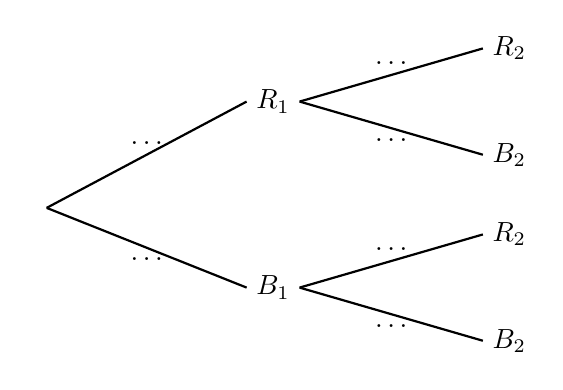
\begin{tikzpicture}[xscale=1,yscale=1]
	% Styles (MODIFIABLES)
	\tikzstyle{fleche}=[-,>=latex,thick]
	\tikzstyle{noeud}=[rounded corners=5pt]
	\tikzstyle{feuille}=[]
	\tikzstyle{commentaire}=[black]
	% Dimensions (MODIFIABLES)
	\def\DistanceInterNiveaux{3}
	\def\DistanceInterFeuilles{1.35}
	% Dimensions calculées (NON MODIFIABLES)
	\def\NiveauA{(0)*\DistanceInterNiveaux}
	\def\NiveauB{(1.0)*\DistanceInterNiveaux}
	\def\NiveauC{(2.0)*\DistanceInterNiveaux}
	\def\NiveauD{(2.750)*\DistanceInterNiveaux}
	\def\NiveauE{(3.5)*\DistanceInterNiveaux}
	\def\InterFeuilles{(-1)*\DistanceInterFeuilles}
	% Noeuds (MODIFIABLES : Styles et Coefficients d'InterFeuilles)
	%	\node[commentaire] (epreuve1) at ({\NiveauB},{(0)*\InterFeuilles}) {\scriptsize Observation};
	%	\node[commentaire] (epreuve2) at ({\NiveauC},{(0)*\InterFeuilles}) {\scriptsize Cause}; 
	%	\node[commentaire] (issues) at ({\NiveauD},{(0)*\InterFeuilles}) {\scriptsize Issues};
	%	\node[commentaire] (probas) at ({\NiveauE},{(0)*\InterFeuilles}) {\scriptsize Probabilités};
	% 
	\node[noeud] (R) at ({\NiveauA},{(2.00)*\InterFeuilles}) {};
	\node[noeud] (Ra) at ({\NiveauB},{(1)*\InterFeuilles}) {$R_1$};
	\node[feuille] (Raa) at ({\NiveauC},{(0.5)*\InterFeuilles}) {$R_2$}; 
	\node[feuille] (Rab) at ({\NiveauC},{(1.5)*\InterFeuilles}) {$ {B_2}$}; 
	\node[noeud] (Rb) at ({\NiveauB},{(2.75)*\InterFeuilles}) {$ {B_1}$};
	\node[feuille] (Rba) at ({\NiveauC},{(2.25)*\InterFeuilles}) {$R_2$}; 
	\node[feuille] (Rbb) at ({\NiveauC},{(3.25)*\InterFeuilles}) {$ {B_2}$}; 
	%
	%	\node[commentaire] (I1) at ({\NiveauD},{(0.5)*\InterFeuilles}) {$A\cap B$}; 
	%	\node[commentaire] (I2) at ({\NiveauD},{(1.5)*\InterFeuilles}) {$A\cap \overline{B}$}; 
	%	\node[commentaire] (I3) at ({\NiveauD},{(2.25)*\InterFeuilles}) {$\overline{A}\cap B$}; 
	%	\node[commentaire] (I4) at ({\NiveauD},{(3.25)*\InterFeuilles}) {$\overline{A}\cap \overline{B}$};
	%	%
	%	\node[commentaire] (P1) at ({\NiveauE},{(0.5)*\InterFeuilles}) {$P(A\cap B)= $}; 
	%	\node[commentaire] (P2) at ({\NiveauE},{(1.5)*\InterFeuilles}){$P(A\cap \overline{B})= $}; 
	%	%	\draw (P2.east) node[anchor=west, commentaire] {Faux négatif};
	%	\node[commentaire] (P3) at ({\NiveauE},{(2.25)*\InterFeuilles}){$P(\overline{A}\cap B)= $}; 
	%	%	\draw (P3.east) node[anchor=west, commentaire] {Faux positif};
	%	\node[commentaire] (P4) at ({\NiveauE},{(3.25)*\InterFeuilles}) {$P(\overline{A}\cap \overline{B})=$}; 
	%	%		\draw[ ultra thick] ({\NiveauE-1},{(3.55)*\InterFeuilles}) -- ({\NiveauE+1},{(3.55)*\InterFeuilles}) ;
	%	%		\node[commentaire] (P5) at ({\NiveauE},{(3.75)*\InterFeuilles})  {\textbf{Total}$=\ldots $}; 
	%	
	% Arcs (MODIFIABLES : Styles)
	\draw[fleche] (R.east)--(Ra.west) node[midway, above]{$\ldots$};
	\draw[fleche] (Ra.east)--(Raa.west) node[midway, above]{$\ldots$};
	\draw[fleche] (Ra.east)--(Rab.west) node[midway, below]{$\ldots$};
	\draw[fleche] (R.east)--(Rb.west) node[midway, below]{$\ldots$};
	\draw[fleche] (Rb.east)--(Rba.west) node[midway, above]{$\ldots$};
	\draw[fleche] (Rb.east)--(Rbb.west) node[midway, below]{$\ldots$};
\end{tikzpicture} 

	\begin{tikzpicture}[xscale=1,yscale=1]
	% Styles (MODIFIABLES)
	\tikzstyle{fleche}=[-,>=latex,thick]
	\tikzstyle{noeud}=[rounded corners=5pt]
	\tikzstyle{feuille}=[]
	\tikzstyle{commentaire}=[black]
	% Dimensions (MODIFIABLES)
	\def\DistanceInterNiveaux{3}
	\def\DistanceInterFeuilles{1.35}
	% Dimensions calculées (NON MODIFIABLES)
	\def\NiveauA{(0)*\DistanceInterNiveaux}
	\def\NiveauB{(1.0)*\DistanceInterNiveaux}
	\def\NiveauC{(2.0)*\DistanceInterNiveaux}
	\def\NiveauD{(2.750)*\DistanceInterNiveaux}
	\def\NiveauE{(3.5)*\DistanceInterNiveaux}
	\def\InterFeuilles{(-1)*\DistanceInterFeuilles}
	% Noeuds (MODIFIABLES : Styles et Coefficients d'InterFeuilles)
	%	\node[commentaire] (epreuve1) at ({\NiveauB},{(0)*\InterFeuilles}) {\scriptsize Observation};
	%	\node[commentaire] (epreuve2) at ({\NiveauC},{(0)*\InterFeuilles}) {\scriptsize Cause}; 
	%	\node[commentaire] (issues) at ({\NiveauD},{(0)*\InterFeuilles}) {\scriptsize Issues};
	%	\node[commentaire] (probas) at ({\NiveauE},{(0)*\InterFeuilles}) {\scriptsize Probabilités};
	% 
	\node[noeud] (R) at ({\NiveauA},{(2.00)*\InterFeuilles}) {};
	\node[noeud] (Ra) at ({\NiveauB},{(1)*\InterFeuilles}) {$R_1$};
	\node[feuille] (Raa) at ({\NiveauC},{(0.5)*\InterFeuilles}) {$R_2$}; 
	\node[feuille] (Rab) at ({\NiveauC},{(1.5)*\InterFeuilles}) {$ {B_2}$}; 
	\node[noeud] (Rb) at ({\NiveauB},{(2.75)*\InterFeuilles}) {$ {B_1}$};
	\node[feuille] (Rba) at ({\NiveauC},{(2.25)*\InterFeuilles}) {$R_2$}; 
	\node[feuille] (Rbb) at ({\NiveauC},{(3.25)*\InterFeuilles}) {$ {B_2}$}; 
	%
	%	\node[commentaire] (I1) at ({\NiveauD},{(0.5)*\InterFeuilles}) {$A\cap B$}; 
	%	\node[commentaire] (I2) at ({\NiveauD},{(1.5)*\InterFeuilles}) {$A\cap \overline{B}$}; 
	%	\node[commentaire] (I3) at ({\NiveauD},{(2.25)*\InterFeuilles}) {$\overline{A}\cap B$}; 
	%	\node[commentaire] (I4) at ({\NiveauD},{(3.25)*\InterFeuilles}) {$\overline{A}\cap \overline{B}$};
	%	%
	%	\node[commentaire] (P1) at ({\NiveauE},{(0.5)*\InterFeuilles}) {$P(A\cap B)= $}; 
	%	\node[commentaire] (P2) at ({\NiveauE},{(1.5)*\InterFeuilles}){$P(A\cap \overline{B})= $}; 
	%	%	\draw (P2.east) node[anchor=west, commentaire] {Faux négatif};
	%	\node[commentaire] (P3) at ({\NiveauE},{(2.25)*\InterFeuilles}){$P(\overline{A}\cap B)= $}; 
	%	%	\draw (P3.east) node[anchor=west, commentaire] {Faux positif};
	%	\node[commentaire] (P4) at ({\NiveauE},{(3.25)*\InterFeuilles}) {$P(\overline{A}\cap \overline{B})=$}; 
	%	%		\draw[ ultra thick] ({\NiveauE-1},{(3.55)*\InterFeuilles}) -- ({\NiveauE+1},{(3.55)*\InterFeuilles}) ;
	%	%		\node[commentaire] (P5) at ({\NiveauE},{(3.75)*\InterFeuilles})  {\textbf{Total}$=\ldots $}; 
	%	
	% Arcs (MODIFIABLES : Styles)
	\draw[fleche] (R.east)--(Ra.west) node[midway, above]{$\tfrac{1}{n+1}$};
	\draw[fleche] (Ra.east)--(Raa.west) node[midway, above]{$\tfrac{1}{n+1}$};
	\draw[fleche] (Ra.east)--(Rab.west) node[midway, below]{$\tfrac{n}{n+1}$};
	\draw[fleche] (R.east)--(Rb.west) node[midway, below]{$\tfrac{n}{n+1}$};
	\draw[fleche] (Rb.east)--(Rba.west) node[midway, above]{$\tfrac{1}{n+1}$};
	\draw[fleche] (Rb.east)--(Rbb.west) node[midway, below]{$\tfrac{n}{n+1}$};
\end{tikzpicture}

$P(M)=P(\text{tirer deux rouges}\cup \text{tirer deux blanches})=\frac{1}{(n+1)^2}+\frac{n^2}{(n+1)^2}=\frac{1+n^2}{(n+1)^2}$. \\
 $P(N)=1-P(M)=\frac{2n}{(n+1)^2}$.\\
L'équation donne $n^2+1=5.05 \times 2n$, soit $n^2-10.1n+1=0$. Une solution à rejeter car \dotfill. On a donc $n=10$.
\end{proof}
\begin{proof}[solution de l'exercice \ref{chapter03:exercise:modelisation11} ]\hfill \\
		\begin{enumerate}[label=\alph*),leftmargin=*]
		\item Aire $=5^2-4\times \frac{1}{2}x(5-x)=25-10x+2x^2$
		\item L'aire est minimale pour $x=\tfrac{10}{4}=2.5$. L'aire minimale est $-\frac{\Delta}{4a}=-\frac{10^2-4\times 25\times 2}{4}=25$.
		\item Résoudre $2x^2-10x+10.88 = 0$  
		\item Résoudre $2x^2-10x+12\geqslant 0$
	\end{enumerate}
\end{proof}
%----------------------------------------------------------------------------------------
%	 
%----------------------------------------------------------------------------------------

\newpage  
%\loadgeometry{fullwidthlayout}  
\loadgeometry{widelayout}  
\pagestyle{empty} % Print headers again  
\KOMAoptions{
	headwidth=textwithmarginpar,
	headsepline=true,
	headsepline= 0.5pt,
	footwidth=textwithmarginpar,
} 
\onehalfspacing
\section{Fiche synthèse fonctions et équations quadratiques}

\paragraph{Savoir faire}

\begin{itemize}
	\item [$\Box$] Identifier une fonction quadratique, l'écrire sous différentes formes : factorisée, développée, canonique
	\item [$\Box$] Résoudre une équation ou une inéquation du second degré 
	\item [$\Box$] Donner l'allure de la courbe représentant une fonction du second degré, préciser les variations et extrema de la fonction
\end{itemize}

\paragraph{Discriminant et Forme canonique}

\begin{definition}
	On appelle fonction quadratique toute fonction $P$ définie sur $\mathbb{R}$ par une expression de la forme $P(x)=ax^2+bx+c$ où $a$, $b$, $c$ sont des réels et $a \neq 0$. 
\end{definition}

\begin{definition}
	Le \textbf{discriminant} du trinôme $ax^2+bx+c$ est le réel noté $\Delta$ défini par :
	\setlength{\abovedisplayskip}{3pt}
	\setlength{\belowdisplayskip}{3pt}
	 $$\Delta=b^2-4ac$$
\end{definition}

\begin{definition}
	La \textbf{forme canonique} de $ax^2+bx+c$ est
	\setlength{\abovedisplayskip}{3pt}
	\setlength{\belowdisplayskip}{3pt}
%	 $$a\left[\left(x+\frac{b}{2a}\right)^2-\frac{\Delta}{4a^2}\right]=a\left(x+\frac{b}{2a}\right)^2-\frac{\Delta}{4a}$$
	 \begin{align*}
	 	a\left[\left(x+\frac{b}{2a}\right)^2-\frac{\Delta}{4a^2}\right]&=a\left(x+\frac{b}{2a}\right)^2-\frac{\Delta}{4a}\\
	 	&= a(x-\upalpha)^2\quad +\upbeta && \upalpha=- \frac{b}{2a} \quad\text{et}\quad \upbeta=- \frac{\Delta}{4a} 
	 	\end{align*}
\end{definition}

\begin{figure*}[!h] 
	\parbox{0.31\linewidth}{
		\begin{tikzpicture}[xscale=0.65, yscale=0.3 ]
			%----------------------- 
			\tkzSetUpPoint[size=3, fill=black]
			\tkzfctset{tan style/.style={->,>=latex, color=red, line width=1.2pt}}  
			\tkzInit[xmin=-4,xmax=4,ymin=-7,ymax=7,xstep=1.0, ystep=1.0  ];
			%	\tkzGrid[color=gray, line width=0.5pt,]
			%	\begin{scope}[dashed] 
				%		\tkzGrid[sub,subxstep=1, subystep=1,color=gray, line width=0.5pt, ]
				%	\end{scope}  
			\tkzDrawX[  noticks, font=\scriptsize, line width=2pt, label=$x$, above =5pt  ] 
			\tkzDrawY[  noticks,  font=\scriptsize, line width=2pt , up space=0.2pt, label={$y$}, right=5pt, ]  
			%	\tkzLabelXY[orig = false,  font=\scriptsize]
			%	\tkzRep[color  = Maroon,line width = 2pt, posxlabel=below, posylabel=left, xnorm=1, ynorm=1]
			%----------------------- 
			\def\a{1}
			\def\b{1.5}
			\def\c{2}
			
			\tkzFct[ domain = -5.0:5.0, line width=1.2pt,   color=blue]{(\a*(\x-\b)**2+\c)}     
			%----------------------- 
			\def\a{-1}
			\def\b{-1.5}
			\def\c{-2}
			
			\tkzFct[ domain = -5.0:5.0, line width=1.2pt,   color=blue]{(\a*(\x-\b)**2+\c)}    
			%-----------------------  
		\end{tikzpicture}  
	}
	\parbox{0.31\linewidth}{
		\begin{tikzpicture}[xscale=0.65, yscale=0.3 ]
			%----------------------- 
			\tkzSetUpPoint[size=3, fill=black]
			\tkzfctset{tan style/.style={->,>=latex, color=red, line width=1.2pt}}  
			\tkzInit[xmin=-4,xmax=4,ymin=-7,ymax=7,xstep=1.0, ystep=1.0  ];
			%	\tkzGrid[color=gray, line width=0.5pt,]
			%	\begin{scope}[dashed] 
				%		\tkzGrid[sub,subxstep=1, subystep=1,color=gray, line width=0.5pt, ]
				%	\end{scope}  
			\tkzDrawX[  noticks, font=\scriptsize, line width=2pt, label=$x$, above =5pt  ] 
			\tkzDrawY[  noticks,  font=\scriptsize, line width=2pt , up space=0.2pt, label={$y$}, right=5pt, ]  
			%	\tkzLabelXY[orig = false,  font=\scriptsize]
			%	\tkzRep[color  = Maroon,line width = 2pt, posxlabel=below, posylabel=left, xnorm=1, ynorm=1]
			%----------------------- 
			\def\a{-1}
			\def\b{1.2}
			\def\c{0}
			
			\tkzFct[ domain = -5.0:5.0, line width=1.2pt,   color=blue]{(\a*(\x-\b)**2+\c)}    
			%-----------------------  
			\def\a{1}
			\def\b{-1.2}
			\def\c{0}
			
			\tkzFct[ domain = -5.0:5.0, line width=1.2pt,   color=blue]{(\a*(\x-\b)**2+\c)}    
			%-----------------------  
		\end{tikzpicture}  
	}
	\parbox{0.31\linewidth}{
		\begin{tikzpicture}[xscale=0.65, yscale=0.3 ]
			%----------------------- 
			\tkzSetUpPoint[size=3, fill=black]
			\tkzfctset{tan style/.style={->,>=latex, color=red, line width=1.2pt}}  
			\tkzInit[xmin=-5,xmax=5,ymin=-7,ymax=7,xstep=1.0, ystep=1.0  ];
			%	\tkzGrid[color=gray, line width=0.5pt,]
			%	\begin{scope}[dashed] 
				%		\tkzGrid[sub,subxstep=1, subystep=1,color=gray, line width=0.5pt, ]
				%	\end{scope}  
			\tkzDrawX[  noticks, font=\scriptsize, line width=2pt, label=$x$, above =5pt  ] 
			\tkzDrawY[  noticks,  font=\scriptsize, line width=2pt , up space=0.2pt, label={$y$}, right=5pt, ]  
			%	\tkzLabelXY[orig = false,  font=\scriptsize]
			%	\tkzRep[color  = Maroon,line width = 2pt, posxlabel=below, posylabel=left, xnorm=1, ynorm=1]
			%----------------------- 
			\def\a{-1}
			\def\b{2.0}
			\def\c{2}
			
			\tkzFct[ domain = -5.0:5.0, line width=1.2pt,   color=blue]{(\a*(\x-\b)**2+\c)}    
			%-----------------------   
			\def\a{1}
			\def\b{-2.0}
			\def\c{-2}
			
			\tkzFct[ domain = -5.0:5.0, line width=1.2pt,   color=blue]{(\a*(\x-\b)**2+\c)}    
			%-----------------------  
		\end{tikzpicture}  
	}
	\caption{Les 3 différents cas: (1) $P(x)=ax^2+bx+c$ ne s'annule pas et ne change pas de signe, (2) $P(x)=ax^2+bx+c$ s'annule mais ne change pas de signe, (3) change de signe 2 fois }
\end{figure*}
\paragraph{Équation du second degré}\hfill 

\noindent On cherche à résoudre l'équation sous \textbf{forme standard} $ax^2+bx+c=0$. On note $\mathcal{S}$ l'ensemble des solutions que l'on nomme \og \textbf{racines} \fg \, du polynome.

\noindent \textbf{Si la résolution n'est pas immédiate}, on \textbf{peut} appliquer la méthode suivante : 
\begin{enumerate}[label=\textbullet,leftmargin=*]
	\item On commence par calculer $\Delta=b^2-4ac$
	\item  Si $\Delta<0$ alors $\mathcal{S}=\emptyset$ (aucune racine).
	\item  Si $\Delta=0$ alors $\mathcal{S}=\lbrace r  \rbrace$ où $r_1=r_2=-\frac{b}{2a}$ (racine double).
	\item Si $\Delta>0$ alors $\mathcal{S}=\lbrace r_1;r_2 \rbrace$ où $r_1=\frac{-b-\sqrt{\Delta}}{2a}$ et $r_2=\frac{-b+\sqrt{\Delta}}{2a}$
\end{enumerate}


\newpage 
\paragraph{Signe du trinôme}

\noindent La résolution d'une inéquation du second degré est liée à l'étude du signe du trinôme.

\begin{enumerate}[label=\textbullet,leftmargin=*]
	\item  Si $\Delta<0$ alors pour tout réel $x$, $ax^2+bx+c$ est du signe de $a$, et \textbf{n'est pas factorisable}.
	\begin{center}
		\begin{tikzpicture}
			%\tikzset{  double style/.style = {double,very thick,double distance=2pt}}
			\tikzset{  double style/.style = {double,thick,double distance=2pt}}
			\tkzTabInit[lgt = 3.5, espcl =3.0, color, colorC = blue!15, colorL = green!15]{$x$ / 1 ,  Signe de $ax^2+bx+c$/ 1.5  }{$-\infty$    , $+\infty$} 
			\tkzTabLine{t, \text{signe de $a$},t}% 
		\end{tikzpicture}  
	\end{center}
	
	\item Si $\Delta=0$ alors pour tout réel $x \neq r$, $ax^2+bx+c=a(x-r)^2$ est du signe de $a$.
	
	\begin{center}
		\begin{tikzpicture}
			%\tikzset{  double style/.style = {double,very thick,double distance=2pt}}
			\tikzset{  double style/.style = {double,thick,double distance=2pt}}
			\tkzTabInit[lgt = 3.5, espcl =3.0, color, colorC = blue!15, colorL = green!15]{$x$ / 1 ,  Signe de $ax^2+bx+c$/ 1.5  }{$-\infty$ ,$r$  , $+\infty$} 
			\tkzTabLine{t,\text{signe de $a$},z,\text{signe de $a$},t}% 
		\end{tikzpicture}   
	\end{center}
	
	\item  Si $\Delta>0$ alors $ax^2+bx+c=a(x-r_1)(x-r_2)$ est du signe de $a$ à l'extérieur des racines :
	
	\begin{center}
		\begin{tikzpicture}
			%\tikzset{  double style/.style = {double,very thick,double distance=2pt}}
			\tikzset{  double style/.style = {double,thick,double distance=2pt}}
			\tkzTabInit[lgt = 3.5, espcl =3.0, color, colorC = blue!15, colorL = green!15]{$x$ / 1 ,  Signe de $ax^2+bx+c$/ 1.5  }{$-\infty$ ,$r_1$ ,$r_2$ , $+\infty$} 
			\tkzTabLine{t,\text{signe de $a$},z,\text{signe de $-a$},z,\text{signe de $a$},t}% 
		\end{tikzpicture}  
	\end{center}
	\ding{42} Attention ! Ici $r_1$ et $r_2$ doivent être classés du plus petit au plus grand.
	
\end{enumerate}

\paragraph{Variation de la fonction} 
La fonction quadratique $P$ définie par $P(x)=ax^2+bx+c$ ($a \neq 0$).\\
$P$ est monotone sur $\interval[open left,scaled]{-\infty}{-\dfrac{b}{2a}}$ et sur $\interval[open right,scaled]{-\dfrac{b}{2a}}{\infty}$.

\noindent La courbe représentative de la fonction $P$ est une \textbf{parabole} dont les branches sont tournées vers le haut si $a>0$ et vers le bas si $a<0$. Le sommet de la parabole a pour coordonnées $\left(\upalpha=\dfrac{-b}{2a};\upbeta=\dfrac{-\Delta}{4a}\right)$. \\
La parabole admet pour axe de symétrie la droite $\mathcal{D} \colon x=-\dfrac{b}{2a}$.
\\
\begin{enumerate}[label=\textbullet,leftmargin=*]
	\item  Si $a>0$ alors $P$  admet un \textbf{minimum}   $\upbeta-\dfrac{\Delta}{4a}$ atteint en $\upalpha=-\dfrac{b}{2a}$. 
\begin{center}
	\begin{tikzpicture}
		%\tikzset{  double style/.style = {double,very thick,double distance=2pt}}
		\tikzset{  double style/.style = {double,thick,double distance=2pt}}
		\tkzTabInit[lgt = 3.5, espcl =2.5, color, colorC = blue!15, colorL = green!15]{$x$ / 1 ,$ax^2+bx+c$ / 2.0    }{$-\infty$ ,$-\frac{b}{2a}$ , $+\infty$} 
		\tkzTabVar{+/$+\infty$  ,- /$-\frac{\Delta}{4a}$,  +/ $+\infty$}  
	\end{tikzpicture} 
\end{center} 
	\item  $a>0$ alors $P$  admet un \textbf{maximum}   $\upbeta=-\dfrac{\Delta}{4a}$ atteint en $\upalpha=-\dfrac{b}{2a}$
\end{enumerate}

\begin{center} 
	\begin{tikzpicture}
%\tikzset{  double style/.style = {double,very thick,double distance=2pt}}
\tikzset{  double style/.style = {double,thick,double distance=2pt}}
\tkzTabInit[lgt = 3.5, espcl =2.5, color, colorC = blue!15, colorL = green!15]{$x$ / 1 ,$ax^2+bx+c$ / 2.0    }{$-\infty$ ,$-\frac{b}{2a}$ , $+\infty$} 
\tkzTabVar{-/$-\infty$  ,+ /$-\frac{\Delta}{4a}$,  -/ $-\infty$}  
\end{tikzpicture}
\end{center} 
\noindent 


    
  


%----------------------------------------------------------------------------------------
%	 
%----------------------------------------------------------------------------------------
\end{document}